% Local preview compatibility; also valid with pdfLaTeX.
\RequirePackage[OT1]{fontenc}
\documentclass[journal,twoside]{IEEEtran}
\usepackage{amsmath,amssymb,bm}
\usepackage{graphicx,booktabs,array,multirow}
\usepackage[noadjust]{cite}
\usepackage{url}
\usepackage{stfloats,balance}
\renewcommand{\dbltopfraction}{0.92}
\renewcommand{\topfraction}{0.92}
\renewcommand{\bottomfraction}{0.85}
\renewcommand{\floatpagefraction}{0.75}
\renewcommand{\dblfloatpagefraction}{0.75}
\setlength{\dbltextfloatsep}{12pt plus 2pt minus 2pt}
\setlength{\textfloatsep}{10pt plus 2pt minus 2pt}
\renewcommand{\textfraction}{0.07}
\usepackage[final]{microtype}
\usepackage[hidelinks]{hyperref}
\graphicspath{{figures/}}
\newcommand{\wrap}{\operatorname{wrap}}
\newcommand{\sinc}{\operatorname{sinc}}
\newcommand{\dist}{\operatorname{dist}}
\newcommand{\clip}{\operatorname{clip}}
\newcommand{\pos}[1]{\left[#1\right]_+}
\newcommand{\ours}{Rolling-WB-V2.1}
\allowdisplaybreaks[1]
\hypersetup{pdftitle={Morphology-Aware Rolling Whole-Body Planning for Aerial Continuum Manipulation in Confined Spaces}}
\newif\ifhardwareplaceholders
\hardwareplaceholderstrue % Set false to hide future-data layout reservations.
\usepackage{placeins}
\begin{document}
\raggedbottom
\title{Morphology-Aware Rolling Whole-Body Planning for Aerial Continuum Manipulation in Confined Spaces}
\author{Author Names Omitted for Anonymous Review}
\maketitle

% Chinese comments provide a paragraph-level drafting companion; the PDF is English.
\begin{abstract}
% CN: 本文以形态感知滚动全身规划为主线，分别说明感知与规划的验证范围，并保留正式实验数据。
% CN:柔性臂弯曲会同时改变空中连续体机械臂的空间占据范围和质量分布，因此在受限空间中，仅规划无人机本体的运动是不充分的。本文提出一种形态感知的滚动全身规划方法，将无人机位置、偏航角、单段连续体形态以及轨迹分段时间进行联合优化。方法首先通过几何引导初始化选择候选通道构型，再在有限在线计算预算内利用 B 样条对全身轨迹进行细化。候选轨迹还需经过独立的密集验证器检查其可行性，并通过连续性感知门控或可选的五次多项式桥接完成相邻滚动窗口之间的轨迹切换。作为形态反馈前端，视觉--应变估计器将动作捕捉监督训练的应变形态预测与经过无人机基座运动补偿的视觉观测进行融合，以在视觉退化条件下持续提供柔性臂形态反馈。感知鲁棒性通过分阶段视觉退化、遮挡和失效实验进行评估，实验过程中同步采集视觉与应变测量数据；滚动规划框架则在 PX4/Gazebo 闭环环境中采用二阶柔性臂响应模型，在 90 个严格配对场景中完成 450 次试验。所提规划器完成 89/90 个任务，成功率为 98.9%，而表现最好的对比方法完成 68/90 个任务，成功率为 75.6%；在 Hard 场景中，本方法成功率为 96.7%，最佳对比方法为 40.0%。规划时间 P95 为 3.697 s，且未观察到规划截止期违约。早期与修订接管版本的配对比较报告了单位路径长度平移 Jerk 能量中位降低 72.8%，单因素归因仍需独立接管消融。上述结果支持在低动态受限空间任务中，将连续体形态纳入全身联合规划，并在滚动轨迹切换前进行独立验证和连续接管。

Arm bending changes both the occupied volume and mass distribution of an aerial continuum manipulator, making vehicle-only planning insufficient in confined spaces. We present a morphology-aware rolling planner that jointly optimizes UAV position, yaw, single-section continuum morphology, and segment timing. Geometry-guided initialization selects candidate passage configurations, and finite-budget B-spline refinement improves the resulting whole-body trajectory. A separate dense validator checks candidate feasibility, while a continuity-aware gate and an optional quintic bridge authorize transitions between rolling windows. A complementary visual--strain estimator combines motion-capture-supervised strain prediction with base-motion-compensated vision to provide morphology feedback under visual degradation. Sensing robustness was evaluated through staged visual-degradation, occlusion, and loss experiments with synchronously acquired visual and strain measurements, while the rolling planning framework was evaluated in 450 PX4/Gazebo closed-loop trials across 90 paired scenarios using a second-order morphology-response model. The planner completed 89/90 tasks (98.9\%), compared with 68/90 (75.6\%) for the strongest baseline; hard-scenario success was 96.7\% versus 40.0\%. Planning-time P95 was 3.697~s, with no observed deadline miss. A paired comparison of the earlier and revised handoff versions reported a 72.8\% median reduction in translational jerk energy per unit path length. A hardware demonstration further illustrates compact passage configurations, arm redeployment, and object handling within a single task. These results support joint morphology planning and validated trajectory switching for low-dynamic confined-space tasks.
\end{abstract}
\begin{IEEEkeywords}
Aerial manipulation, continuum robots, whole-body planning, visual--strain fusion, trajectory handoff.
\end{IEEEkeywords}

\section{Introduction}\label{sec:intro}
% CN: 受限空间中需要规划的是整机占据区域；引言不以“刚性臂不能折叠”为前提。
% CN:
%\section{引言}

%空中机械臂将机器人检测与作业能力扩展到地面平台难以到达的区域~\cite{ollero2022survey}。当通道尺寸逐渐接近机器人整机尺度时，系统运动是否可行，不再只取决于无人机本体，而取决于飞行器、机械臂以及末端工具共同形成的空间占据范围。对于安装在无人机下方的单段连续体机械臂，其弯曲会同时改变工具端位置、机械臂扫掠几何以及整机组合质心（CoM）。因此，在连续穿越多个受限通道时，连续体机械臂的形态必须与无人机运动统一考虑。

%这一问题带来两个相互耦合的困难。首先，由于负载变化和结构非理想特性会影响柔性臂的实际响应，驱动指令并不能始终准确代表其真实弯曲状态。末端眼在手视觉能够提供外部几何反馈，但遮挡和较差的图像质量可能导致视觉跟踪中断；相比之下，应变传感不依赖外部视野，可以提供互补的形态观测。其次，即使无人机本体路径可行，也并不意味着机械臂能够保持无碰撞构型。联合规划需要在不同弯曲方向之间进行搜索，同时控制在线计算开销。此外，即使相邻滚动窗口生成的局部轨迹分别满足可行性要求，其边界状态及其导数仍可能存在不匹配，从而在重规划切换时产生突变的控制指令。

%针对上述问题，本文采用图~\ref{fig:framework} 所示的系统架构。一个统一的形态状态接口将基于置信度自适应的视觉--应变形态估计模块与滚动全身规划器连接起来。规划器首先搜索几何可行的轨迹种子，然后联合细化轨迹形状与时间分配，并将生成的候选轨迹提交给独立的密集验收模块。随后，单独的轨迹接管阶段进一步判断新候选轨迹能否直接替换当前正在执行的命令轨迹，或者是否需要通过经过重新验证的桥接轨迹完成切换。本文的一个核心思想就是明确区分“生成一条可行候选轨迹”和“授权该轨迹进入实际执行”这两个过程。

%本文的主要贡献如下。

%1) 提出一种滚动全身联合规划方法，将无人机位置与偏航、单段连续体机械臂形态以及非均匀样条的时间参数统一建模。通过几何引导初始化和局部连续细化，在有限计算预算内组织非凸全身轨迹搜索。

%2) 提出一种轨迹执行授权机制，将候选轨迹的密集可行性验证与新旧轨迹之间的切换验收显式分离。通过边界速率继承、相位匹配以及可选的五次多项式桥接，减小独立生成的相邻滚动窗口之间的状态和导数不连续。

% CN: 贡献3：构建与规划器兼容的视觉--应变形态反馈前端，将独立监督训练的应变形态估计与经过无人机基座运动补偿的视觉观测进行融合，并针对普通角度变量和圆周角变量采用置信度自适应的信息加权。最终形成统一的形态状态接口，为后续全身规划和轨迹接管提供连续体形态表示。
\IEEEPARstart{A}{erial} manipulators extend robotic inspection and intervention to locations that are difficult to reach from the ground~\cite{ollero2022survey}. When passage dimensions approach the scale of the robot, feasibility depends on the occupied volume of the vehicle, arm, and distal tool. For a single-section continuum arm mounted beneath a UAV, bending changes the tool position, swept arm geometry, and combined center of mass (CoM). Its morphology must therefore be considered together with vehicle motion when negotiating successive confined passages.

% CN: 从空间耦合引出实际形态反馈，再引出在线非凸求解与接管问题。
Two coupled difficulties arise. First, actuation commands cannot always represent realized bending because loading and structural nonidealities affect the arm response. End-eye vision offers geometric feedback, but occlusion and poor image quality can interrupt tracking; strain sensing provides a complementary observation that does not require an external view. Second, a feasible vehicle path need not admit a collision-free arm configuration. Joint planning must search among different bending directions while controlling online computation. Even when successive local plans are individually feasible, their boundary states and derivatives can differ, producing abrupt command changes during replanning.

% CN: 论文以规划和连续接管为核心，感知作为可连接的前端；不把分开验证写成端到端验证。
We address these difficulties with the architecture in Fig.~\ref{fig:framework}, supported by the modular platform described in Sec.~\ref{sec:hardware_architecture}. A morphology interface connects confidence-adaptive visual--strain estimation to a rolling whole-body planner. The planner searches for a geometric seed, jointly refines trajectory and timing, and submits the candidate to a dense acceptance check. A separate handoff stage then determines whether the candidate can replace the active command trajectory directly or through a revalidated bridge. This distinction between generating a feasible candidate and authorizing its execution is central to the method.

The contributions are as follows.
\begin{enumerate}
\item A rolling whole-body formulation couples UAV position and yaw with single-section continuum morphology and nonuniform spline timing. Geometry-guided initialization and local refinement organize the search within a finite computation budget.
\item A trajectory-authorization mechanism separates dense candidate validation from transition acceptance. Boundary-rate inheritance, phase matching, and optional quintic bridging address discontinuities between independently generated windows.
\item A morphology-feedback frontend combines independently supervised strain estimation with base-motion-compensated vision using confidence-adaptive linear and circular information weighting. The resulting morphology-state interface provides a unified representation for downstream whole-body planning and trajectory handoff.
\end{enumerate}
% CN: 图1 形态感知的滚动全身规划系统架构。单段连续体机械臂采用单一恒曲率圆弧模型，并刚性安装在无人机下方。四通道表面应变传感器提供柔性臂形态观测，末端 D435 相机与夹爪构成刚性组件，其姿态随柔性臂末端切线方向变化。离线阶段利用动作捕捉系统提供监督标签，训练基于应变的形态预测模型。在线运行过程中，根据当前视觉跟踪质量，将应变形态估计与经过无人机基座运动补偿的视觉观测进行自适应融合，为后续规划器提供柔性臂形态反馈。滚动规划器联合细化无人机运动、连续体形态和轨迹时间分配。每条候选轨迹在执行前均需经过独立的密集验证和轨迹接管授权；当相邻滚动窗口无法直接连续接管时，可采用五次多项式 C2 桥接完成轨迹过渡。图中的虚线状态连接表示形态估计模块与全身规划模块之间的统一形态状态接口。
\begin{figure*}[!tb]
\centering
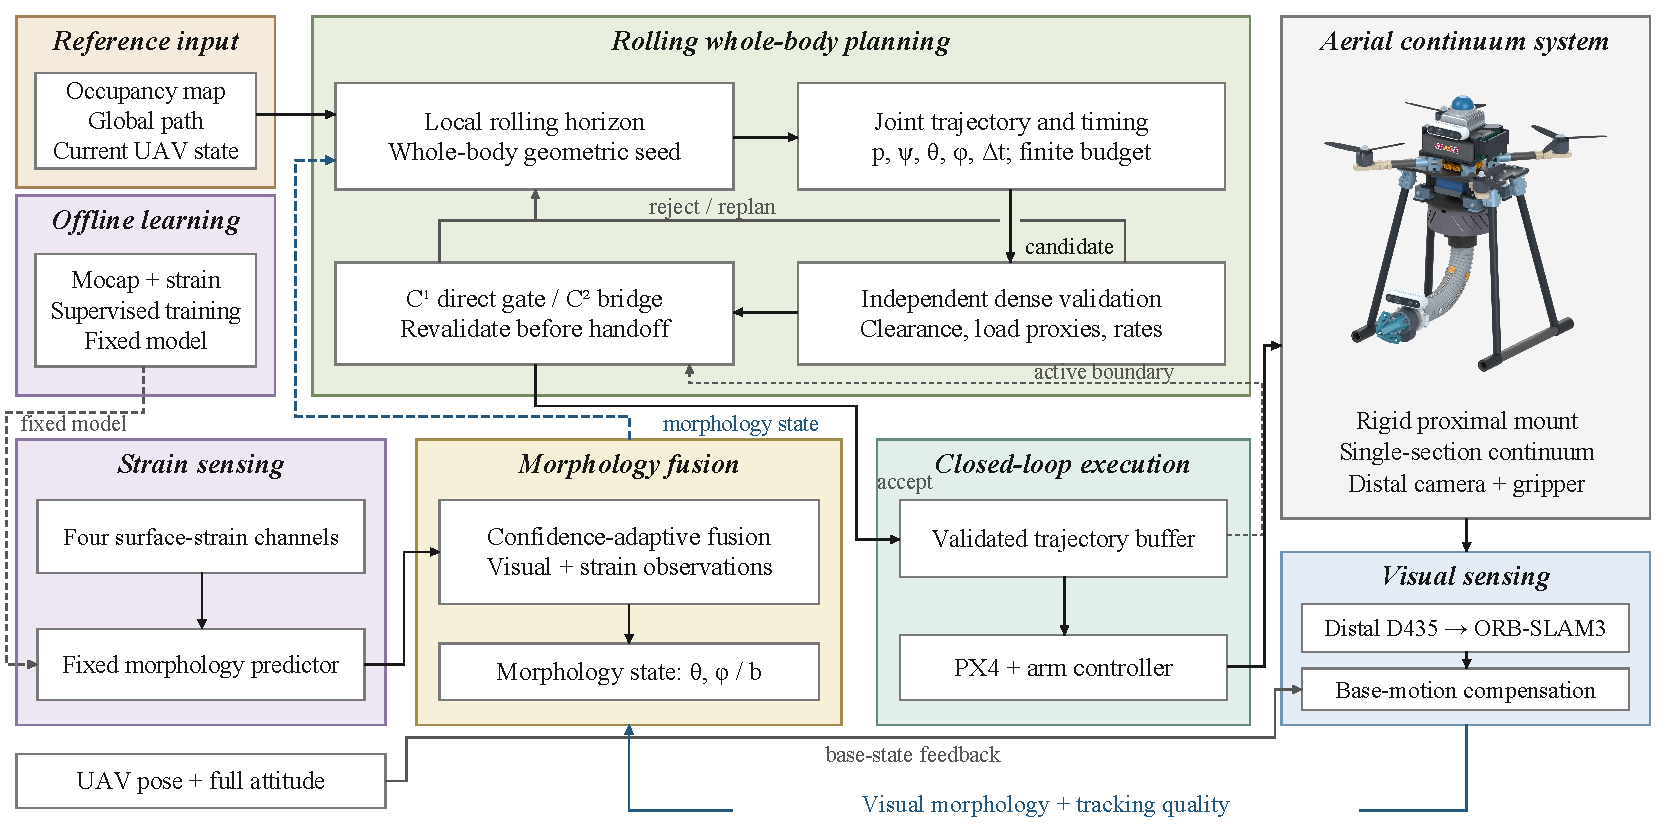
\includegraphics[width=\textwidth]{system_framework_journal.pdf}
\caption{Morphology-aware rolling whole-body architecture. The planner jointly refines vehicle motion, continuum morphology, and segment timing within a finite budget. Dense candidate validation and continuity-aware handoff form separate acceptance stages; a quintic bridge is revalidated before admission to the trajectory buffer. Rejected candidates or transitions leave the active trajectory in place. Offline-trained strain prediction and base-motion-compensated distal vision produce a confidence-adaptive morphology estimate through the dashed state interface. UAV pose and full attitude support rolling initialization and visual compensation. The physical platform is rendered from the native CAD assembly.}
\label{fig:framework}
\end{figure*}

\section{Related Work}\label{sec:related}
\subsection{Aerial Manipulation and Coupled Planning}
% CN: 依据原论文界定差异；不把结构适配基线写成原作者代码复现。
% CN: 空中机械臂系统的轨迹规划需要同时协调飞行平台与机械臂运动，并考虑控制可行性对轨迹选择的影响。已有工作中，AeCoM 展示了结合 IMU 建模与防松弛机制的空中连续体机械臂平台；Aerial Elephant Trunk 进一步面向杂乱和受限环境开展了灵巧操作研究。另一方面，也有研究将多旋翼无人机与刚性 Delta 机械臂进行一体化规划，并统一考虑航路点、碰撞以及动力学约束。与上述工作不同，本文聚焦于单段 PCC 连续体机械臂，并强调在有限在线计算预算下进行滚动全身搜索，同时显式处理相邻局部轨迹之间的接管与切换问题。
Aerial manipulation requires coordinated platform and arm motion, with control feasibility influencing trajectory choice~\cite{ollero2022survey,tognon2018controlaware}. AeCoM demonstrated an aerial continuum platform with IMU-based modeling and tendon-slacking prevention~\cite{peng2023aecom}; the Aerial Elephant Trunk system developed dexterous manipulation in cluttered and constrained environments~\cite{peng2025aet}. Integrated planning has also coupled a multirotor and a rigid delta arm under waypoint, collision, and dynamic constraints~\cite{deng2025wholebody}. The present work considers a single PCC section and emphasizes finite-budget rolling search together with the acceptance of transitions between local trajectories.


Recent articulated aerial manipulators provide complementary perspectives. QuadHand combines robot-centric signed distance fields with coupled base--arm trajectory optimization for close-proximity interaction~\cite{jin2026quadhand}. Recurrent visual policies address acquisition and lifting under partial observations~\cite{jin2026visualrl}, while scene-scale VLA systems use measured-progress alignment to connect asynchronously generated action chunks and local behaviors~\cite{guo2026scenevla}. Our focus is the deformable single-section morphology, finite-budget rolling search, and validation of both candidate trajectories and their transitions in confined passages.

\subsection{Continuum Morphology Feedback}
% CN: 视觉—应变互补已有相关工作；本研究的区别在独立离线监督、空中基座运动补偿及下游规划接口。
% CN: 恒曲率模型能够以较紧凑的方式描述连续体机器人的几何形态，但由于实际结构响应会受到迟滞、负载和装配误差等因素影响，真实构型往往仍需要通过直接感知获得。已有相关研究包括基于学习的构型估计、基于光纤的形状感知，以及传感器标定与结构变形联合估计等方法。视觉--应变融合也已经被用于眼在手连续体机器人的状态反馈与控制。本文沿用视觉与应变信息互补这一基本思路，但采用独立的离线动作捕捉监督来训练应变形态估计器，并显式补偿空中平台基座运动对末端视觉观测的影响。最终估计器输出连续体机械臂的两个弯曲形态坐标，用于描述柔性臂相对于其基座的形态；该模块不负责无人机位姿估计，也不构建新的 SLAM 后端。
Constant-curvature models give a compact geometric description of continuum robots~\cite{webster2010pcc}, while realized configuration may require direct sensing~\cite{shi2017survey}. Relevant approaches include learned configuration estimation~\cite{hyatt2019config}, fiber-based shape sensing~\cite{ryu2014fbg,lun2019surface}, and joint calibration and deformation estimation~\cite{alambeigi2020scade}. Visual--strain fusion has already been demonstrated for eye-in-hand continuum-robot feedback and control~\cite{wang2020eyeinhand,wang2023visualstrain}. We use this established complementarity with offline motion-capture supervision and explicit compensation for aerial-base motion. The estimator supplies two bending coordinates; it does not replace the UAV pose estimator or introduce a new SLAM backend.

% CN: 针对多旋翼飞行器，已有多项轨迹生成与优化方法能够有效获得平滑运动，例如多项式轨迹生成、EGO-Planner 和 GCOPTER。对于更一般的非凸构型空间，采样式规划与连续轨迹优化则分别从离散搜索和连续优化角度提供了互补思路。对于搭载连续体机械臂的空中机器人而言，柔性臂会引入随形态变化的连续骨架几何，使碰撞模型不再只由无人机本体决定。本文的方法首先通过离散搜索获得几何可行的初始化结果，再通过连续优化进行轨迹细化，并进一步将候选轨迹本身的可行性检查与滚动窗口之间的轨迹切换验收分开处理。由于在线搜索受有限计算预算约束，本文不对所得结果作全局最优性保证。


\subsection{Trajectory Generation and Validation}
% CN: 车辆轨迹优化、连续体采样规划与全身滚动接管分别承担不同问题。
Polynomial trajectory generation~\cite{mellinger2011minsnap}, EGO-Planner~\cite{zhou2021egoplanner}, and GCOPTER~\cite{wang2022gcopter} provide effective tools for smooth multicopter motion. Sampling-based planning~\cite{karaman2011sampling,meng2022rrtstar} and continuous optimization~\cite{schulman2014trajopt} address complementary aspects of nonconvex configuration spaces. An attached continuum arm adds a morphology-dependent backbone to the collision model. Our approach combines discrete initialization and continuous refinement, then subjects the result and its rolling transition to separate acceptance checks. No global-optimality guarantee is claimed for the finite-budget search.

\section{System Model and Planning Problem}\label{sec:model}
\subsection{Hardware Architecture and Modular Integration}
\label{sec:hardware_architecture}
The platform comprises a quadrotor, a rigid proximal mount, a single-section continuum arm, and a distal camera--gripper assembly (Fig.~\ref{fig:hardware_architecture}). The hardware arrangement distinguishes vehicle-fixed sensing and computation from the deforming arm and its rigid distal tool.

\begin{figure*}[!t]
\centering
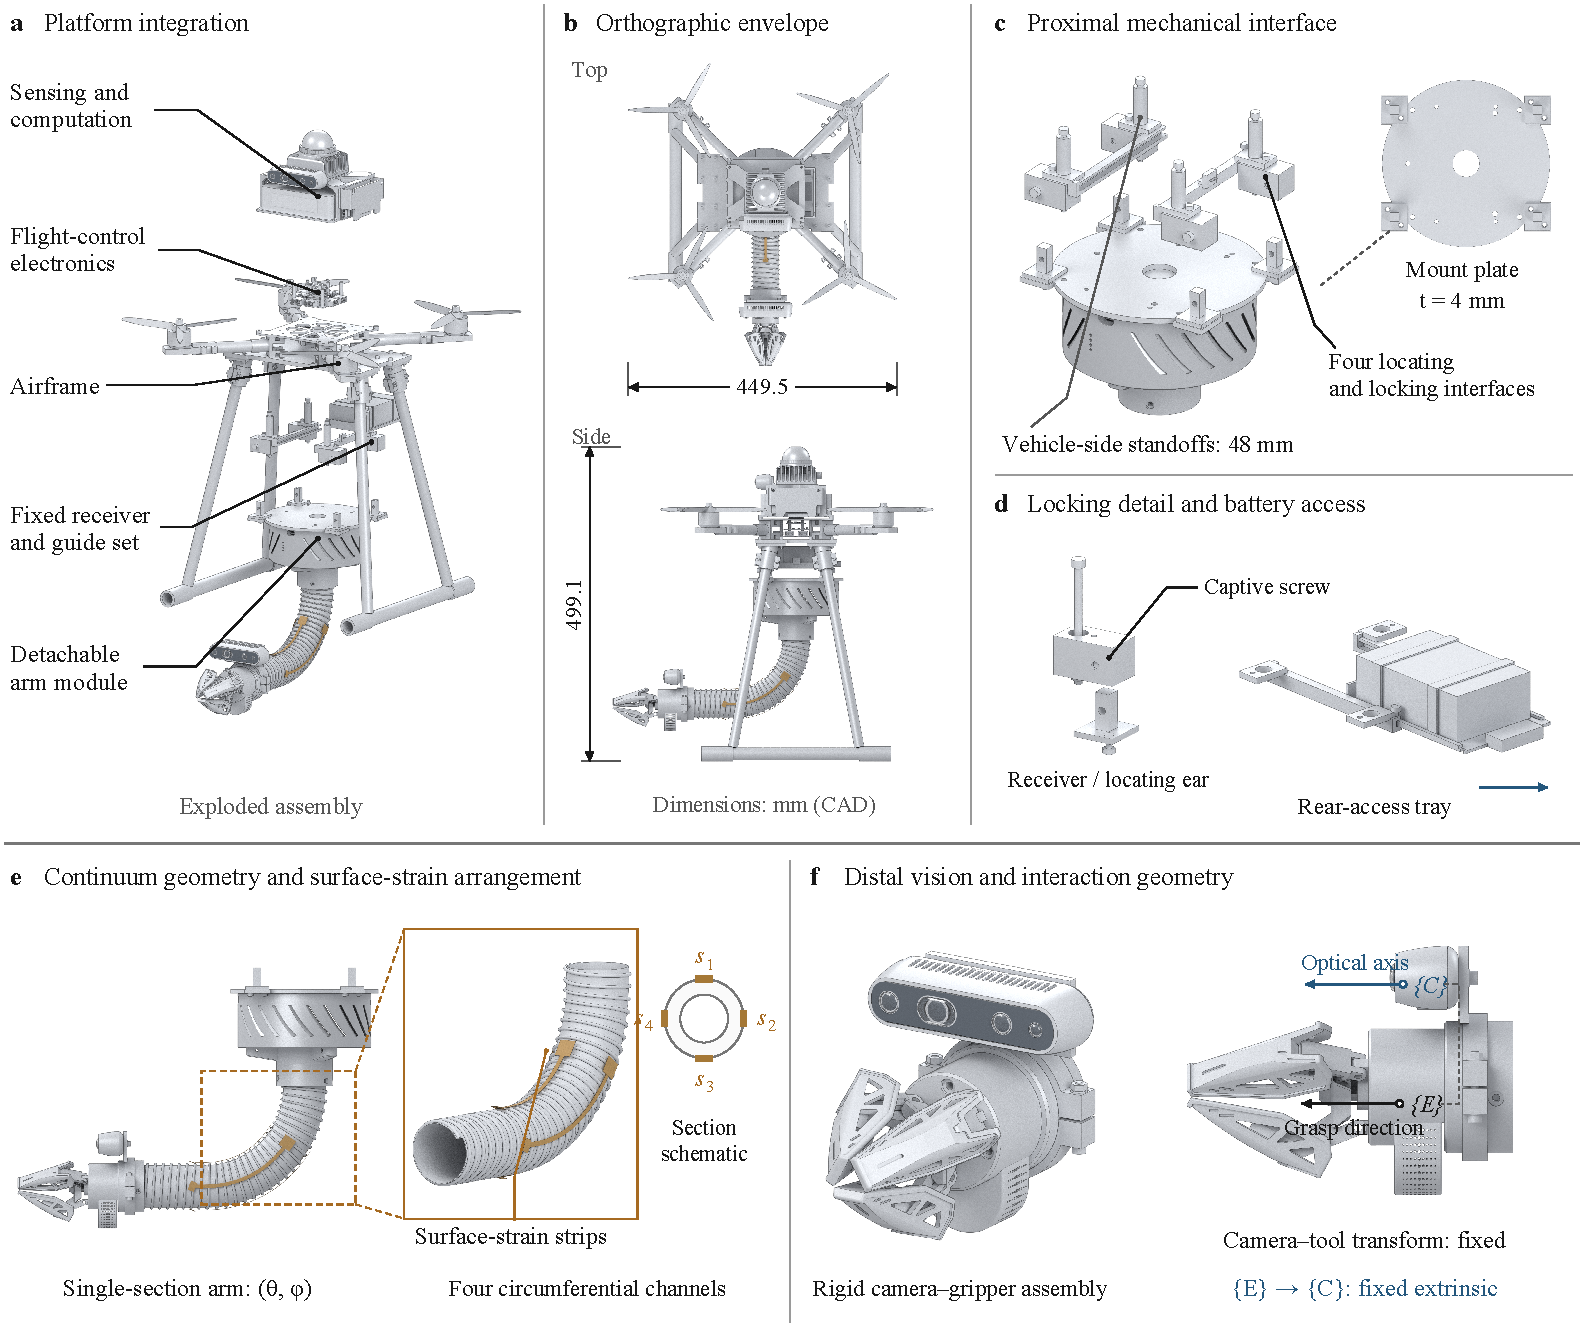
\includegraphics[width=\textwidth]{hardware_architecture_journal.pdf}
\caption{Platform integration, mechanical interfaces, and morphology sensing. (a) Native-CAD exploded assembly separating sensing/computation, flight electronics, airframe, fixed receivers, and the removable arm module. (b) Orthographic views and the envelope of the shown CAD configuration (mm). (c) Mount plate and vehicle-side standoffs. (d) Local locking interface and independent rear-access battery tray. (e) Single-section continuum module, enlarged surface-strain placement, and a schematic four-channel cross-section. (f) Distal assembly and side projection showing the fixed camera--tool relationship. All structural views use the same native CAD geometry and rendering convention. Exploded offsets illustrate assembly relationships. The LiDAR-equipped layout is the configuration for the planned map-registered flight study.}
\label{fig:hardware_architecture}
\end{figure*}

\textit{Vehicle and attachment:} The upper stack accommodates scene-facing sensors and an onboard computer, while the flight controller and power electronics occupy the central airframe. Underbody receivers engage the arm-side mounting plate through locking interfaces. The battery tray is accessed independently from the rear. Once installed, the arm mount defines a fixed vehicle-to-arm transformation; module removal is a maintenance configuration.

\textit{Morphology and distal sensing:} Four circumferential surface-strain channels observe arm deformation. The distal D435 and three-finger gripper are joined through a rigid clamp, preserving the camera-to-tool extrinsic as the continuum section bends. These observations are complementary to the body-mounted sensors: distal vision and strain support morphology estimation, while the LiDAR-equipped layout provides the scene-sensing configuration for the map-registered hardware study in Sec.~\ref{sec:hardware}.

\textit{Planning interface:} The hardware is represented by fixed mounting transforms, a morphology-dependent backbone, and the rigid distal assembly. UAV position and yaw combine with $(\theta,\phi)$ to form the six-dimensional planning state. This physical decomposition motivates the coupled occupancy model and the base-motion compensation developed below.


\subsection{Configuration and Coordinate Frames}
% CN: 明确坐标变换方向。D435仅在直臂参考构型时向下，其光轴与末端之间是固定外参关系。
The system comprises a multirotor, a vertically suspended single-section continuum arm, a distal tool assembly carrying a D435 camera, and four circumferential strain channels. Frames $\{W\}$, $\{U\}$, $\{B\}$, $\{E\}$, and $\{C\}$ denote the world, UAV, proximal arm mount, distal tool, and camera frames. A rotation ${}^{A}\mathbf R_D$ maps coordinates from $\{D\}$ into $\{A\}$. The mount position ${}^{U}\mathbf p_B$, mount rotation ${}^{U}\mathbf R_B$, and camera-to-tool extrinsic ${}^{C}\mathbf R_E$ are fixed. The camera looks downward in the straight reference configuration and subsequently rotates with the distal assembly; it is not world-stabilized.

% CN: 单段不等于单自由度。theta非负；phi在theta=0时没有唯一值。
The constant-curvature section has length $L_a$, bending magnitude $0\le\theta\le\theta_{\max}<\pi$, and bending-plane angle $\phi\in S^1$. Define
\begin{equation}
\mathbf q_a=[\theta,\phi]^{\mathrm T},\qquad
\mathbf b=\theta[\cos\phi,\sin\phi]^{\mathrm T}.
\label{eq:morphology_state}
\end{equation}
For $\|\mathbf b\|>0$, $\theta=\|\mathbf b\|$ and $\phi=\operatorname{atan2}(b_y,b_x)$. At $\mathbf b=\mathbf0$, the arm is straight and $\phi$ is undefined; a retained numerical angle does not imply an observable bending plane. Angular differences use $\wrap(a)=\operatorname{atan2}(\sin a,\cos a)$. Both yaw and $\phi$ are locally unwrapped for spline interpolation.

\subsection{Single-Arc Geometry}
% CN: 用sinc恒等式代替有限阈值处切换到直线的近似，保留零弯曲极限与小角度连续性。
Let $s\in[0,L_a]$ be arc length and $u=\theta s/L_a$. With $\sinc(u)=\sin(u)/u$ and $\sinc(0)=1$, the centerline is
\begin{equation}
{}^{B}\mathbf r_c(s)=s
\begin{bmatrix}
\frac{u}{2}\sinc^2(u/2)\cos\phi\\
\frac{u}{2}\sinc^2(u/2)\sin\phi\\
\sinc(u)
\end{bmatrix},\quad
{}^{B}\mathbf t_e=
\begin{bmatrix}
\sin\theta\cos\phi\\\sin\theta\sin\phi\\\cos\theta
\end{bmatrix}.
\label{eq:pcc_geometry}
\end{equation}
This is algebraically identical to the circular-arc expression for nonzero curvature and tends continuously to $[0,0,s]^{\mathrm T}$ as $\theta\to0$. Each configuration is one planar circular arc; $\phi$ rotates that plane and does not create an additional section or an inflection.

% CN: 规划只优化位置与偏航；近悬停几何采用偏航近似，感知补偿仍使用完整实测姿态。
The planned state is
\begin{equation}
\mathbf x=[\mathbf p_u^{\mathrm T},\psi,\theta,\phi]^{\mathrm T}\in\mathbb R^6,
\label{eq:planning_state}
\end{equation}
where $\mathbf p_u$ and $\psi$ are UAV position and yaw. The planning geometry uses a quasi-hover yaw approximation, $\mathbf R_z(\psi)$; roll and pitch remain controlled by the flight controller. With rigid proximal length $L_b$, distal offset $L_e$, and $\mathbf e_z=[0,0,1]^{\mathrm T}$,
\begin{align}
{}^{W}\mathbf p_c(s)&=\mathbf p_u+\mathbf R_z(\psi)
\left[{}^{U}\mathbf p_B+{}^{U}\mathbf R_B
\big(L_b\mathbf e_z+{}^{B}\mathbf r_c(s)\big)\right],\label{eq:world_centerline}\\
{}^{W}\mathbf p_e&={}^W\mathbf p_c(L_a)
+L_e\mathbf R_z(\psi){}^{U}\mathbf R_B{}^{B}\mathbf t_e.
\label{eq:world_tool}
\end{align}
The $L_b$ offset is applied once: $\{B\}$ is the proximal mount, and $\mathbf r_c$ describes the flexible section relative to its root. The full measured UAV attitude is used separately for visual base-motion compensation in Sec.~\ref{sec:estimation}.

\subsection{Collision and Flight-Load Screening}
% CN: 保留正式基准的采样几何，不虚构解析胶囊碰撞代码；区分物理包络、地图查询和安全余量。
The benchmark queries the complete set of modeled components. Let $\mathcal P_u(\mathbf x)$ sample the cylindrical body/rotor envelope, and let $\mathcal P_a(\mathbf x)$ sample the rigid base, flexible centerline, and distal tool. The occupied-map representation is $\mathcal O$. Its distance query gives the sampled clearances
\begin{equation}
\begin{aligned}
d_u(\mathbf x)&=\min_{\mathbf p\in\mathcal P_u(\mathbf x)}\dist(\mathbf p,\mathcal O),\\
d_a(\mathbf x)&=\min_{\mathbf p\in\mathcal P_a(\mathbf x)}\dist(\mathbf p,\mathcal O)-r_a.
\end{aligned}
\label{eq:clearance}
\end{equation}
Here $r_a$ is the shared tubular radius used for the arm and tool approximation in the benchmark. The body radius is already represented in $\mathcal P_u$ and is not subtracted again. Positive thresholds $d_{u,\min}$ and $d_{a,\min}$ provide additional clearance. These sampled quantities approximate occupied-volume separation; they are not exact solid-body distances. In particular, physical deployment requires the distal envelope to enclose the complete camera and gripper housing, as well as allowance for attitude and tracking errors.

% CN: 所有质心在世界系中；水平质心偏移属于重力负担代理，不等于任意倾斜时的推力轴距离。
For uniform flexible-section mass, its centroid and the system CoM are
\begin{equation}
\begin{aligned}
\mathbf r_a&=\frac{1}{L_a}\int_0^{L_a}{}^W\mathbf p_c(s)\,\mathrm ds,\\
\mathbf r_{\mathrm{com}}&=\frac{\sum_{j\in\{u,b,a,e\}}m_j\mathbf r_j}{m_\Sigma},
\qquad m_\Sigma=\sum_jm_j,\\
d_{\mathrm{com}}&=\|\mathbf P_{xy}(\mathbf r_{\mathrm{com}}-\mathbf r_u)\|_2.
\end{aligned}
\label{eq:com}
\end{equation}
All centroids are expressed in $\{W\}$; $\mathbf r_u$ is the UAV reference centroid and $\mathbf P_{xy}$ selects the horizontal components. The distal mass includes its attached equipment. Equal-arc-length quadrature evaluates the flexible centroid. In quasi-hover, $m_\Sigma g d_{\mathrm{com}}$ characterizes the magnitude of the gravitational moment about the UAV reference; it is not a separate independent constraint from $d_{\mathrm{com}}$.

% CN: 推力比以悬停重力归一化，而非以电机最大推力归一化。
With $\mathbf a_f=\ddot{\mathbf p}_u+g\mathbf e_z$, the dimensionless load ratio and tilt proxy are
\begin{equation}
r_T=\frac{\|\mathbf a_f\|_2}{g},\qquad
\gamma=\operatorname{atan2}\big(\|\mathbf P_{xy}\mathbf a_f\|_2,
\mathbf e_z^{\mathrm T}\mathbf a_f\big).
\label{eq:flight_proxy}
\end{equation}
Thus $r_T=1$ corresponds to hover, rather than motor saturation. These quantities screen translational load in the low-dynamic regime. They do not include arm-relative inertia, flexible vibration, rotor allocation, or aerodynamic coupling.

\subsection{Rolling Planning Objective}
% CN: Facc是数值验收条件集合，不称为控制不变安全集；优化与验收采用相同阈值而不同采样网格。
At cycle $k$, the planner receives UAV state, morphology feedback, $\mathcal O$, a global geometric reference $\Gamma_g$, and the active validated trajectory. It seeks a timed local trajectory satisfying the acceptance conditions
\begin{equation}
\begin{aligned}
\mathcal F_{\mathrm{acc}}=\{(\mathbf x,\dot{\mathbf x},\ddot{\mathbf x},\dddot{\mathbf p}_u):\;&
d_u\ge d_{u,\min},\ d_a\ge d_{a,\min},\\
&d_{\mathrm{com}}\le d_{\mathrm{com}}^{\max},\\
&r_T^{\min}\le r_T\le r_T^{\max},\\
&\gamma\le\gamma^{\max},\quad g_{\mathrm{kin}}\le0\}.
\end{aligned}
\label{eq:acceptance_set}
\end{equation}
The vector $g_{\mathrm{kin}}$ collects prescribed altitude, translational velocity, acceleration and jerk bounds, yaw-rate/acceleration bounds, and morphology position/rate/acceleration bounds. The search evaluates these conditions at collocation states; an independent grid is used for acceptance. The additional requirement is an admissible transition from the active command trajectory. Neither the sampled feasible set nor the transition gate is claimed to be a control-invariant safety set.

\section{Visual--Strain Morphology Estimation}\label{sec:estimation}
\subsection{Independently Supervised Strain Model}
% CN: 对向通道差先扣零点，并保留安装方向及通道增益；不直接假设As等于单位阵。
Let $\alpha_i=\alpha_0+(i-1)\pi/2$ be the four sensor angles. For channel output $s_i$, baseline $s_i^0$, and curvature $\kappa=\theta/L_a$, a bending-motivated observation model is
\begin{equation}
\begin{aligned}
\bar s_i&=s_i-s_i^0=c_i\kappa\cos(\phi-\alpha_i)+r_i+n_i,\\
\mathbf d&=[\bar s_1-\bar s_3,\bar s_2-\bar s_4]^{\mathrm T}
\approx\mathbf A_s\mathbf b+\boldsymbol\epsilon_s.
\end{aligned}
\label{eq:strain_physics}
\end{equation}
The gain $c_i$ includes transduction and sensor placement; $r_i$ represents residual structural effects and $n_i$ measurement noise. The matrix $\mathbf A_s\in\mathbb R^{2\times2}$ has units of channel output per radian and includes $L_a^{-1}$, channel gains, and $\alpha_0$. It is proportional to the identity only for matched gains and aligned sensor axes. Equation~\eqref{eq:strain_physics} motivates the features, while the deployed mapping is learned from independently measured morphology.

% CN: 动捕测基座和末端刚体，用已标定的工具轴提取单段弯曲；不把驱动指令当监督真值。
During offline calibration, motion capture tracks the arm base and a distal marker frame $\{R\}$ in mocap frame $\{M\}$. With fixed marker-to-tool rotation ${}^{R}\mathbf R_E$,
\begin{equation}
\begin{aligned}
\mathbf t^M&=({}^{M}\mathbf R_B)^{\mathrm T}
{}^{M}\mathbf R_R{}^{R}\mathbf R_E\mathbf e_z,\\
\theta^M&=\operatorname{atan2}\big(\sqrt{(t_x^M)^2+(t_y^M)^2},t_z^M\big),\\
\phi^M&=\operatorname{atan2}(t_y^M,t_x^M).
\end{aligned}
\label{eq:mocap_label}
\end{equation}
The superscript $M$ identifies the measurement source; $\mathbf t^M$ itself is expressed in $\{B\}$. The tool $z$ axis must be calibrated to the distal tangent. The labels describe dominant bending under the single-section assumption and do not identify axial twist.

% CN: 保留原稿的监督目标，补齐维度和直臂附近phi权重；不虚构网络层数或训练样本数。
A regressor $f_\omega:\mathbb R^{d_f}\to\mathbb R^2$ maps normalized strain features $\mathbf u_k$ to $(\hat\theta_k^s,\hat\phi_k^s)$. Features include channel increments and opposite-channel differences. Its stated training objective is
\begin{equation}
\begin{aligned}
\min_\omega\ \sum_{k\in\mathcal D_{\mathrm{tr}}}\big[&
(f_\omega^\theta(\mathbf u_k)-\theta_k^M)^2\\
&+\lambda_\phi w_\phi(\theta_k^M)
\wrap^2(f_\omega^\phi(\mathbf u_k)-\phi_k^M)\big]
+\lambda\|\omega\|_2^2,\\
w_\phi(\theta)&=\min(1,\theta/\theta_\phi)^2.
\end{aligned}
\label{eq:strain_training}
\end{equation}
Here $\mathcal D_{\mathrm{tr}}$ is the training set, $d_f$ the feature dimension, $\theta_\phi>0$ the observability scale, and $\lambda_\phi,\lambda\ge0$ the loss weights. Complete acquisition sessions define the training/validation/test partitions. Held-out residuals supply nominal strain variances; abnormal offsets, saturation, and out-of-distribution measurements reduce strain confidence. Online fusion does not retrain the strain mapping.

\subsection{Base-Motion-Compensated Visual Observation}
% CN: ORB姿态先经世界对齐并扣除无人机基座运动，才能解释为柔性臂形态。
Let $\{O\}$ be the ORB map frame, ${}^{O}\mathbf R_C$ its camera orientation, ${}^{W}\mathbf R_U$ the measured UAV attitude, and ${}^{O}\mathbf R_W$ the world-to-map alignment. Then
\begin{equation}
\begin{aligned}
{}^{O}\mathbf R_B&={}^O\mathbf R_W{}^W\mathbf R_U{}^U\mathbf R_B,\\
\mathbf t^v&=({}^{O}\mathbf R_B)^{\mathrm T}
{}^{O}\mathbf R_C{}^{C}\mathbf R_E\mathbf e_z.
\end{aligned}
\label{eq:visual_rotation}
\end{equation}
The same tangent-to-angle map as in \eqref{eq:mocap_label} gives $(\hat\theta^v,\hat\phi^v)$. Visual information is withheld following map-frame changes until alignment is restored. This observation uses relative orientation; UAV translation is not inferred from arm strain.

% CN: 质量分数是融合启发式量，不称作ORB提供的概率或完整标定后验。
Following ORB-SLAM3 tracking diagnostics~\cite{campos2021orbslam3}, visual quality is modeled using valid-tracking indicator $\delta_k^{\mathrm{track}}$, inlier count $N_{\mathrm{in},k}$, reprojection error $e_{\mathrm{rep},k}$, and observation age $a_k^v$:
\begin{equation}
\begin{aligned}
c_k^v=\delta_k^{\mathrm{track}}\bigg[&\clip\left(
\frac{N_{\mathrm{in},k}-N_{\min}}{N_{\mathrm{ref}}-N_{\min}},0,1\right)\\
&\times\exp(-e_{\mathrm{rep},k}^2/\sigma_e^2-a_k^v/\tau_a)\bigg]^{1/3}.
\end{aligned}
\label{eq:visual_quality}
\end{equation}
The calibration constants satisfy $N_{\mathrm{ref}}>N_{\min}$ and $\sigma_e,\tau_a>0$. For $q\in\{\theta,\phi\}$, visual information is $I_{v,k,q}=(c_k^v)^{\eta_q}/\sigma_{v,0,q}^2$, with $\eta_q>0$, and is set to zero for lost or stale observations. Strain information is $I_{s,k,q}=1/\sigma_{s,k,q}^2$. These confidence-derived quantities determine relative weighting rather than a fully calibrated posterior probability.

\subsection{Angular Fusion and Temporal Filtering}
% CN: theta线性融合、phi圆周融合；信息为零和圆周合向量抵消时必须承认观测不可用。
For positive total information, define $w_{m,k}^q=I_{m,k,q}/(I_{v,k,q}+I_{s,k,q})$ for $m\in\{v,s\}$. The fused observations are
\begin{equation}
\begin{aligned}
\tilde\theta_k&=\sum_mw_{m,k}^{\theta}\hat\theta_k^m,\\
(A_k,B_k)&=\sum_mw_{m,k}^{\phi}(\cos\hat\phi_k^m,\sin\hat\phi_k^m),\\
\tilde\phi_k&=\operatorname{atan2}(B_k,A_k).
\end{aligned}
\label{eq:angular_fusion}
\end{equation}
The circular observation requires $A_k^2+B_k^2>0$. Near cancellation or a straight arm, $\phi$ does not provide a reliable correction. A missing or undefined coordinate is excluded from the measurement update; if both modalities are unavailable, the filter propagates without a new observation. Decreasing visual information shifts weight toward strain without treating a frozen visual estimate as a valid measurement.

% CN: 当前状态转移和观测为线性加圆周创新，准确称为圆周创新卡尔曼滤波；Joseph形式保持协方差对称半正定。
Define $\mathbf z=[\theta,\phi,\dot\theta,\dot\phi]^{\mathrm T}$, $\mathbf F_k=\left[\begin{smallmatrix}\mathbf I_2&\Delta t_k\mathbf I_2\\\mathbf0&\mathbf I_2\end{smallmatrix}\right]$, and $\mathbf H=[\mathbf I_2\ \mathbf0]$. Prediction and correction are
\begin{equation}
\begin{aligned}
\mathbf z_k^-&=\mathbf F_k\mathbf z_{k-1}^+,&
\mathbf P_k^-&=\mathbf F_k\mathbf P_{k-1}^+\mathbf F_k^{\mathrm T}+\mathbf Q_k,\\
\boldsymbol\nu_k&=\begin{bmatrix}\tilde\theta_k-\theta_k^-\\\wrap(\tilde\phi_k-\phi_k^-)\end{bmatrix},&
\mathbf S_k&=\mathbf H\mathbf P_k^-\mathbf H^{\mathrm T}+\mathbf R_k,\\
\mathbf K_k&=\mathbf P_k^-\mathbf H^{\mathrm T}\mathbf S_k^{-1},&
\mathbf z_k^+&=\mathbf z_k^-+\mathbf K_k\boldsymbol\nu_k,\\
\mathbf A_k&=\mathbf I-\mathbf K_k\mathbf H,&
\mathbf P_k^+&=\mathbf A_k\mathbf P_k^-\mathbf A_k^{\mathrm T}
+\mathbf K_k\mathbf R_k\mathbf K_k^{\mathrm T}.
\end{aligned}
\label{eq:kalman}
\end{equation}
Here $\mathbf P$ is state covariance, $\mathbf Q_k$ process covariance, and $\mathbf R_k$ the fused-observation covariance. The local independent-error approximation gives nominal diagonal entries $(I_{v,k,q}+I_{s,k,q})^{-1}$; for $\phi$ this approximation applies only to concentrated angular residuals. The filter uses the available rows of $\mathbf H$ when an observation is excluded. Its role is temporal regularization, not a new nonlinear state estimator. The interface exports $(\hat\theta,\hat\phi)$ and the corresponding $\hat{\mathbf b}$.

\section{Rolling Whole-Body Planning}\label{sec:planning}
\subsection{Local Reference and Boundary State}
% CN: 预测规划完成后的接管位置只是初始化，实际接管仍重新门控；路径进度限制为前向邻域。
The global reference $\Gamma_g=\{\mathbf p^r(\ell),\psi^r(\ell)\}$ supplies passage direction, with $\ell$ denoting arc length. Let $\mathcal T_k^{\mathrm{val}}$ be the active validated trajectory, $\tau_k$ its current phase, $\alpha_k$ its phase rate, and $t_p$ estimated planning latency. Initialization uses
\begin{equation}
\begin{aligned}
\tau_k^p&=\clip(\tau_k+\alpha_kt_p,0,T_k^{\mathrm{val}}),\\
\bar{\mathbf x}_k&=\mathcal T_k^{\mathrm{val}}(\tau_k^p),\qquad
\dot{\bar{\mathbf x}}_k=\alpha_k\mathcal T_k^{\mathrm{val}\prime}(\tau_k^p).
\end{aligned}
\label{eq:prediction}
\end{equation}
Without an active trajectory, measured state initializes the first window. The nearest reference point is sought in a forward neighborhood of the previous progress estimate, and a length-$L_h$ local horizon is cropped. This avoids choosing a distant branch at a reference self-intersection. The latency prediction initializes the successor; the actual switching boundary is checked again when the candidate is ready.

\subsection{Spline Geometry, Timing, and Cost}
% CN: 节点向量两端均夹持，控制点数Nc=Ns+3；sigma具有时间单位，不与机械臂弧长s混用。
Use $N_s$ positive span durations $\Delta=[\Delta t_0,\ldots,\Delta t_{N_s-1}]^{\mathrm T}$, with $t_j=\sum_{r<j}\Delta t_r$ and $T_g=\sum_r\Delta t_r$. The cubic knot vector and nominal trajectory are
\begin{equation}
\begin{aligned}
\mathcal K&=[0,0,0,0,t_1,\ldots,t_{N_s-1},T_g,T_g,T_g,T_g],\\
\mathbf x_g(\sigma)&=\sum_{i=0}^{N_c-1}N_{i,3}(\sigma;\mathcal K)\mathbf c_i,
\qquad N_c=N_s+3.
\end{aligned}
\label{eq:spline}
\end{equation}
The basis functions $N_{i,3}$ are cubic B-splines, $\mathbf c_i\in\mathbb R^6$, and $\mathbf C\in\mathbb R^{N_c\times6}$ stacks the control states. Both endpoints are clamped. The phase $\sigma\in[0,T_g]$ has units of seconds; ordinary rolling successors use unit phase rate. Smooth phase ramps are reserved for task startup and terminal stopping.

% CN: 补齐几何相位到执行时间的链式法则，所有运动约束和jerk均针对执行时间。
For execution time $t$, $\mathbf x(t)=\mathbf x_g(\sigma(t))$ and $\alpha=\dot\sigma$. Primes denote phase derivatives and dots execution-time derivatives:
\begin{equation}
\begin{aligned}
\dot{\mathbf x}&=\alpha\mathbf x_g',\\
\ddot{\mathbf x}&=\alpha^2\mathbf x_g''+\dot\alpha\mathbf x_g',\\
\dddot{\mathbf p}_u&=\alpha^3\mathbf p_g'''
+3\alpha\dot\alpha\mathbf p_g''+\ddot\alpha\mathbf p_g'.
\end{aligned}
\label{eq:chain_rule}
\end{equation}
Ramps must therefore be included in derivative and feasibility checks. A unit-rate successor inherits $\mathbf c_0=\bar{\mathbf x}_k$ and $\mathbf c_1=\mathbf c_0+(\Delta t_0/3)\dot{\bar{\mathbf x}}_k$; it does not restart from zero velocity. Simple interior knots give a $C^2$ nominal spline, with piecewise-defined jerk and one-sided knot limits.

% CN: 目标保持原稿的离散配点平均，不把非均匀配点平均误称为精确时间积分。
For execution-time collocation set $\mathcal S_c$, write $\langle f\rangle_c=|\mathcal S_c|^{-1}\sum_{t\in\mathcal S_c}f(t)$. A monotone progress mapping defines the interpolated local reference $(\bar{\mathbf p}^{r}(t),\bar\psi^r(t))$. The objective is
\begin{equation}
\begin{aligned}
\min_{\mathbf C,\Delta}J={}&w_pJ_p+w_\psi J_\psi+w_jJ_j
+w_{\dot a}J_{\dot a}+w_{\ddot a}J_{\ddot a}\\
&+w_{cl}J_{cl}+w_{cp}J_{cp}+w_TT_g+w_\Delta J_\Delta+w_eJ_e,
\end{aligned}
\label{eq:objective}
\end{equation}
subject to \eqref{eq:acceptance_set}, boundary conditions, and prescribed $0<\Delta t_{\min}\le\Delta t_r\le\Delta t_{\max}$. The terms are
\begin{equation}
\begin{aligned}
J_p&=\langle\|\mathbf p_u-\bar{\mathbf p}^{r}\|^2\rangle_c,\\
J_\psi&=\langle\wrap^2(\psi-\bar\psi^r)\rangle_c,\\
J_j&=\langle\|\dddot{\mathbf p}_u\|^2\rangle_c,\\
J_{\dot a}&=\langle\|\dot{\mathbf q}_a\|^2\rangle_c,\qquad
J_{\ddot a}=\langle\|\ddot{\mathbf q}_a\|^2\rangle_c,\\
J_{cl}&=\langle\pos{d_{u,s}-d_u}^2+\pos{d_{a,s}-d_a}^2\rangle_c,\\
J_{cp}&=\langle(d_{\mathrm{com}}/d_{\mathrm{com}}^{\max})^2\rangle_c,\\
J_\Delta&=\frac{1}{N_s-1}\sum_{r=0}^{N_s-2}(\Delta t_{r+1}-\Delta t_r)^2.
\end{aligned}
\label{eq:cost_terms}
\end{equation}
Here $[a]_+=\max(a,0)$, $d_{u,s}>d_{u,\min}$ and $d_{a,s}>d_{a,\min}$ define soft clearance preferences, and the fixed nonnegative weights account for the different physical units. $J_\Delta=0$ for a single span. These are collocation averages, not exact integral costs.

% CN: 终端目标只在有操作任务的最后窗口启用，Tg是名义跨度总和。
At the nominal endpoint, the terminal cost is
\begin{equation}
\begin{aligned}
J_e={}&\|\mathbf p_g(T_g)-\mathbf p_{u,e}^r\|^2\\
&+\mathbb I_e\big[\lambda_\theta(\theta_g(T_g)-\theta_e)^2
+\lambda_\phi\wrap^2(\phi_g(T_g)-\phi_e)\\
&\hspace{16mm}+\lambda_t\|\mathbf p_e(\mathbf x_g(T_g))-\mathbf p_e^*\|^2\big].
\label{eq:terminal}
\end{aligned}
\end{equation}
The indicator $\mathbb I_e$ activates the desired morphology $(\theta_e,\phi_e)$ and tool target $\mathbf p_e^*$ only for a terminal manipulation window. The local UAV target is $\mathbf p_{u,e}^r$. The $T_g$ term penalizes nominal duration, while soft clearance and CoM terms rank candidates without replacing the hard acceptance thresholds.

\subsection{Geometric Seed and Finite-Budget Refinement}
% CN: 先离散选通道和形态，再细化控制状态；种子点不是可直接执行的轨迹。
Sparse reference nodes with low body/arm clearance or CoM margin define risk intervals. Around node $i$, the search evaluates
\begin{equation}
\mathcal C_i=\{(\mathbf p_i^r+\delta\mathbf p_m,\psi_i^r,\theta_n,\phi_l)\},
\label{eq:candidates}
\end{equation}
where $\delta\mathbf p_m$, $\theta_n$, and $\phi_l$ are finite displacement and morphology candidates. The current bending plane is tried first; additional planes are opened if it cannot support a connected feasible sequence or the refined trajectory fails validation. A beam-limited search retains low-cost, morphology-diverse states according to
\begin{equation}
D_i(c)=J_i^{\mathrm{node}}(c)+\min_{c'\in\mathcal B_{i-1}}
\{D_{i-1}(c')+J_i^{\mathrm{edge}}(c',c)\}.
\label{eq:beam}
\end{equation}
Node costs rank reference deviation, clearance, and morphology; edge costs include adjacent-state changes and interpolated collision checks. $\mathcal B_{i-1}$ is the retained beam. The selected sequence initializes spline controls $\mathbf C^0$ and times $\Delta^0$, rather than being executed directly.

% CN: 低维变形只作用于自由控制点，首两点单独重建，消除原式同时冻结又优化的矛盾。
Only free control states are deformed using $\mathbf B\in\mathbb R^{(N_c-2)\times M}$ and $\boldsymbol\Xi\in\mathbb R^{M\times6}$:
\begin{equation}
\begin{aligned}
\mathbf C_{2:}&=\mathbf C^0_{2:}+\mathbf B\boldsymbol\Xi,\\
\mathbf c_0&=\bar{\mathbf x}_k,\qquad
\mathbf c_1=\mathbf c_0+\frac{\Delta t_0}{3}\dot{\bar{\mathbf x}}_k.
\end{aligned}
\label{eq:local_basis}
\end{equation}
The notation $2:$ selects rows with indices $2,\ldots,N_c-1$. Whenever the first span changes, $\mathbf c_1$ is reconstructed. This preserves the physical boundary rate while optimizing timing.

% CN: 模式搜索解决距离查询非光滑问题；罚项仅排序，不能替代最终验收。
Let $\boldsymbol\zeta=[\operatorname{vec}(\boldsymbol\Xi)^{\mathrm T},\Delta^{\mathrm T}]^{\mathrm T}$. Projected coordinate pattern search evaluates $\Pi_{\mathcal Z}(\boldsymbol\zeta\pm\rho_j\mathbf e_j)$, where $\mathcal Z$ is the bounded parameter domain and $\rho_j$ a coordinate step. A merit function $\widetilde J=J+\mu\sum_m[-s_m]_+^2$, with constraint slack $s_m$ and penalty weight $\mu\ge0$, orders trial points. Search terminates within its allotted budget; only a subsequently validated candidate can be authorized.

\subsection{Dense Validation and Transition Authorization}
% CN: 保留正式实现记录中时间、平移、theta、phi四项，加入至少一次细分；不声称端点差能够界定区间内最大扫掠。
The validator regenerates the trajectory on a grid separate from the optimizer. For coarse execution-time interval $[t_i,t_{i+1}]$, it uses
\begin{equation}
\begin{aligned}
n_i&=\max\!\left(1,\left\lceil\max\{r_t,r_p,r_\theta,r_\phi\}\right\rceil\right),\\
r_t&=\frac{t_{i+1}-t_i}{\delta_t},\quad
r_p=\frac{\|\Delta\mathbf p_i\|}{\delta_p},\\
r_\theta&=\frac{|\Delta\theta_i|}{\delta_\theta},\quad
r_\phi=\frac{|\wrap(\Delta\phi_i)|}{\delta_\phi}.
\end{aligned}
\label{eq:validation}
\end{equation}
All limits $\delta_\bullet$ are positive. Each added state is checked against \eqref{eq:acceptance_set}, including yaw-dependent whole-body geometry and execution-time derivatives. Endpoint differences alone do not bound interior motion, and the count has no separate yaw-excursion term. Thus the fixed temporal resolution remains essential; this procedure provides sampled acceptance evidence, not a continuous-time collision certificate.

% CN: 接管比较坐标qh中使用b；用排序尺度和门控阈值分别定义，避免二者混同。
A validated candidate is compared with the currently issued command in continuity coordinates $\boldsymbol\xi=[\mathbf p_u^{\mathrm T},\psi,\mathbf b^{\mathrm T}]^{\mathrm T}$. Its mismatch vector $\mathbf e_h(\tau)$ contains position, wrapped yaw, bending vector, linear velocity, yaw rate, and bending-vector rate differences, normalized by fixed ranking scales. Over a bounded forward candidate interval $\mathcal I_s$,
\begin{equation}
\tau_s^*=\arg\min_{\tau\in\mathcal I_s}\|\mathbf e_h(\tau)\|_\infty.
\label{eq:phase_match}
\end{equation}
The actual switching boundary must satisfy a separate componentwise gate:
\begin{equation}
\begin{bmatrix}
\|\Delta\mathbf p\|\\|\wrap(\Delta\psi)|\\\|\Delta\mathbf b\|\\
\|\Delta\mathbf v\|\\|\Delta\dot\psi|\\\|\Delta\dot{\mathbf b}\|
\end{bmatrix}
\preceq
\begin{bmatrix}
\varepsilon_p\\\varepsilon_\psi\\\varepsilon_b\\
\varepsilon_v\\\varepsilon_{\dot\psi}\\\varepsilon_{\dot b}
\end{bmatrix}.
\label{eq:handoff_gate}
\end{equation}
Finite tolerances give approximate first-order matching. The benchmark label ``C1 direct handoff'' refers to this gate, not exact mathematical $C^1$ equality at a splice.

% CN: 五次桥接在[p,psi,b]坐标匹配两端0/1/2阶导数；必须转回物理形态并检查整段及两个连接点。
If direct acceptance fails, a duration-$T_{\mathrm{br}}>0$ quintic bridge $\mathbf h(t)=\sum_{r=0}^{5}\mathbf a_rt^r$ is constructed in $\boldsymbol\xi$. With old command boundary $\boldsymbol\xi_o$ and candidate boundary $\boldsymbol\xi_c$,
\begin{equation}
\begin{aligned}
\mathbf h^{(j)}(0)&=\boldsymbol\xi_o^{(j)},&
\mathbf h^{(j)}(T_{\mathrm{br}})&=\boldsymbol\xi_c^{(j)},\quad j=0,1,2.
\end{aligned}
\label{eq:bridge_boundary}
\end{equation}
Derivatives come from the issued and candidate commands, including phase scaling. Yaw endpoints use a common unwrapped branch. The bridge is mapped back to physical morphology and validated with its endpoint joins and candidate suffix; smooth interpolation alone does not establish collision or rate feasibility. When \eqref{eq:bridge_boundary} is met, the splice is $C^2$ in command coordinates $\boldsymbol\xi$. This is not a claim of $C^2$ measured UAV--arm motion or of an observable $\phi$ at zero bending.

% CN: 更新缓存时保留的是旧轨迹未执行部分；制动/悬停不是无需验收的天然安全动作。
Let $V_c$ denote full-candidate validation, $G$ the direct gate, $V_b$ bridge-and-join validation, and $\mathcal T_c^{\mathrm{tail}}$ the candidate suffix starting at $\tau_s^*$. The future command buffer becomes
\begin{equation}
\mathcal T^{\mathrm{new}}=
\begin{cases}
\mathcal T_c^{\mathrm{tail}},&V_c\land G,\\
\mathcal H_{\mathrm{br}}\oplus\mathcal T_c^{\mathrm{tail}},&V_c\land\neg G\land V_b,\\
\mathcal T_o^{\mathrm{remain}},&\text{otherwise},
\end{cases}
\label{eq:cache}
\end{equation}
where $\oplus$ denotes time-aligned concatenation. Candidate generation runs while the old buffer is executed. Its remaining duration must cover planning, validation, switching, and reserve:
\begin{equation}
T_{\mathrm{remain}}>T_{\mathrm{plan}}+T_{\mathrm{validate}}
+T_{\mathrm{switch}}+T_{\mathrm{reserve}}.
\label{eq:buffer}
\end{equation}
Deceleration or hold is admissible only if its continuation also satisfies the acceptance conditions. Repeated rejection or exhaustion without an authorized continuation is treated as failure; retaining an old trajectory alone does not guarantee indefinite safety.

\section{Experimental Evaluation}\label{sec:experiments}
\subsection{Setup and Matched Protocol}
% CN: 感知鲁棒性与规划性能分别采用相应的实验协议进行验证。感知实验在同步采集视觉与应变数据的过程中分阶段引入视觉退化，用于评估融合权重迁移和形态估计连续性。规划性能则在 PX4/Gazebo 闭环环境中进行验证，在 90 个严格配对场景中共完成 450 次试验，并通过统一的 $(\theta,\phi)$ 形态状态接口采用二阶柔性臂响应模型描述形态动态。表~\ref{tab:parameters} 给出了主要平台与规划参数。

Morphology-feedback robustness and planning performance were evaluated under their corresponding experimental protocols. The sensing experiments introduced staged visual degradation while visual and strain measurements were synchronously acquired to assess modality reweighting and estimation continuity. Planning performance was evaluated in 450 PX4/Gazebo closed-loop trials across 90 paired scenarios, with a second-order arm-response model providing morphology dynamics through the common $(\theta,\phi)$ interface. A complementary hardware demonstration illustrates morphology-coordinated passage and object handling (Sec.~\ref{sec:hardware}). Table~\ref{tab:parameters} lists the principal platform and planning parameters for the simulation benchmark.

\begin{table}[t]
\centering
\caption{Principal benchmark parameters.}
\label{tab:parameters}
\small
\begin{tabular}{lc@{\quad}lc}
\toprule
Parameter & Value & Parameter & Value\\\midrule
Arm length & 0.22 m & Arm radius & 0.034 m\\
Maximum $\theta$ & $120^\circ$ & Total mass & 2.25 kg\\
UAV radius & 0.28 m & CoM bound & 0.08 m\\
Body/arm margin & 0.10/0.07 m & Horizon & 3.0 m\\
Spline controls & 8 & Command period & 0.05 s\\
Validation $\delta_p$ & 0.03 m & $\delta_\theta/\delta_\phi$ & $3^\circ/5^\circ$\\
Planning deadline & 15 s & Tilt bound & $15^\circ$\\\bottomrule
\end{tabular}
\end{table}

% CN: 90场景的任务种子与规划器随机种子是不同概念；仅保留材料所载的场景协议。
The 90 paired scenarios covered Passage-Sweep, Multi-Passage, and Clutter-Reach, each at Easy, Medium, and Hard difficulty. Each family--difficulty cell contained ten tasks with fixed scenario seeds 11--20. Planner input was a common RGB-D/SLAM occupancy snapshot; unknown voxels were occupied, and hidden geometric truth was reserved for post-hoc auditing. The supplied protocol used a Latin-rotation method order within each scenario cell. Each method was evaluated once per scenario; these task replications do not quantify repeated-run variability of a randomized planner on one fixed task.

% CN: 明确三类文献基线为结构适配实现，并保留共享条件。
\emph{Fixed} followed the common reference with one development-set-selected morphology. \emph{AET-Seq.} adapted the waypoint/configuration decomposition of~\cite{peng2025aet}, fixing the UAV reference before solving a single-section morphology corridor. \emph{WB-RRT*} adapted RRT*~\cite{karaman2011sampling,meng2022rrtstar} to the coupled six-dimensional state and continued improvement after finding a solution. \emph{Global-WB} adapted the integrated batch structure of~\cite{deng2025wholebody}, replacing the delta-arm state with PCC morphology. These were structured adaptations, not the original authors' implementations. All five methods shared map input, task reference, hard constraints, terminal tolerances, low-level control, and a 15-s per-attempt wall-clock deadline. Failed and timed-out runs remained in the success denominator.

% CN: 规划裕度和事后实测验收阈值分别列明，不能混写为同一阈值。
A successful trial required at least 1.0~s terminal dwell with tool error at most 0.08~m, available measured whole-body states, and no abort or unsafe event. Post-hoc swept-clearance limits were 0.06~m for the body and 0.02~m for the arm; these differ from the planning margins in Table~\ref{tab:parameters}. Maximum position-tracking error was limited to 0.25~m and continuous hold to 20~s. Exceeding the preregistered consecutive-rejection threshold also constituted failure. Planning latency and deadline statistics included all logged attempts, whether accepted or rejected.

% CN: 给出指标的单位和处理方式；不凭空指定原稿未披露的滤波窗口整数样本数。
For each successful trial, clearance was the minimum audited separation along the measured trajectory; P05 denotes the fifth percentile of these trial minima. Tracking RMSE used time-aligned measured and issued UAV positions. Commanded velocities were deduplicated, resampled at 20~Hz, and differentiated twice with the same third-order Savitzky--Golay procedure and nominal 0.5-s window. With commanded path length $L_c>0$,
\begin{equation}
E_{j/L}=\frac{1}{L_c}\int_{t_0}^{t_f}\|\hat{\mathbf j}_u(t)\|_2^2\,\mathrm dt,
\qquad [E_{j/L}]=\mathrm{m\,s^{-5}}.
\label{eq:jerk_metric}
\end{equation}
This filtered command metric does not measure raw physical jerk or mathematical impulses at discontinuities. Success rates used Wilson 95\% intervals and exact paired McNemar tests. Descriptive continuous summaries used each method's successful trials; paired continuous inference used only the 54 tasks completed by all methods, with bootstrap median differences, Holm-corrected Wilcoxon tests, and rank-biserial effect sizes.

\subsection{Whole-Body Success and Computation}
% CN: 主表保留全部指定指标；P95恢复3.697的已给精度，避免把非最优值加粗。
\begin{table*}[t]
\centering
\caption{Results on 90 paired scenarios (450 trials). Task time, tracking RMSE, jerk energy, and tip error are medians on each method's successful trials; clearances are P05 of per-trial minima. Planning P95 and deadline misses include all attempts.}
\label{tab:main}
\small\setlength{\tabcolsep}{3.1pt}
\begin{tabular}{lcccccccc}
\toprule
Method & Success, \% [95\% CI] & Task & Plan P95 & Deadline & Body/arm P05 & Track RMSE & $E_{j/L}$ & Tip error\\
 & & (s) & (s) & miss (\%) & (m) & (m) & (m s$^{-5}$) & (m)\\\midrule
Fixed & 61.1 [50.8, 70.5] & 130.72 & 2.94 & 0.00 & 0.2324/0.1490 & 0.0214 & 0.0867 & 0.0176\\
AET-Seq. & 67.8 [57.6, 76.5] & 98.06 & 10.44 & 0.00 & 0.2295/0.1436 & 0.0285 & 0.2734 & 0.0140\\
WB-RRT* & 75.6 [65.8, 83.3] & 168.55 & 13.02 & 0.00 & 0.1793/0.1390 & 0.0195 & 0.0619 & 0.0155\\
Global-WB & 65.6 [55.3, 74.6] & 99.68 & 10.39 & 2.25 & 0.2286/0.1434 & 0.0270 & 0.2574 & 0.0144\\
\textbf{\ours} & \textbf{98.9 [94.0, 99.8]} & 103.62 & 3.697 & 0.00 & 0.1827/0.1442 & 0.0240 & 0.1263 & 0.0129\\\bottomrule
\end{tabular}
\end{table*}

\begin{figure*}[!tb]
\centering
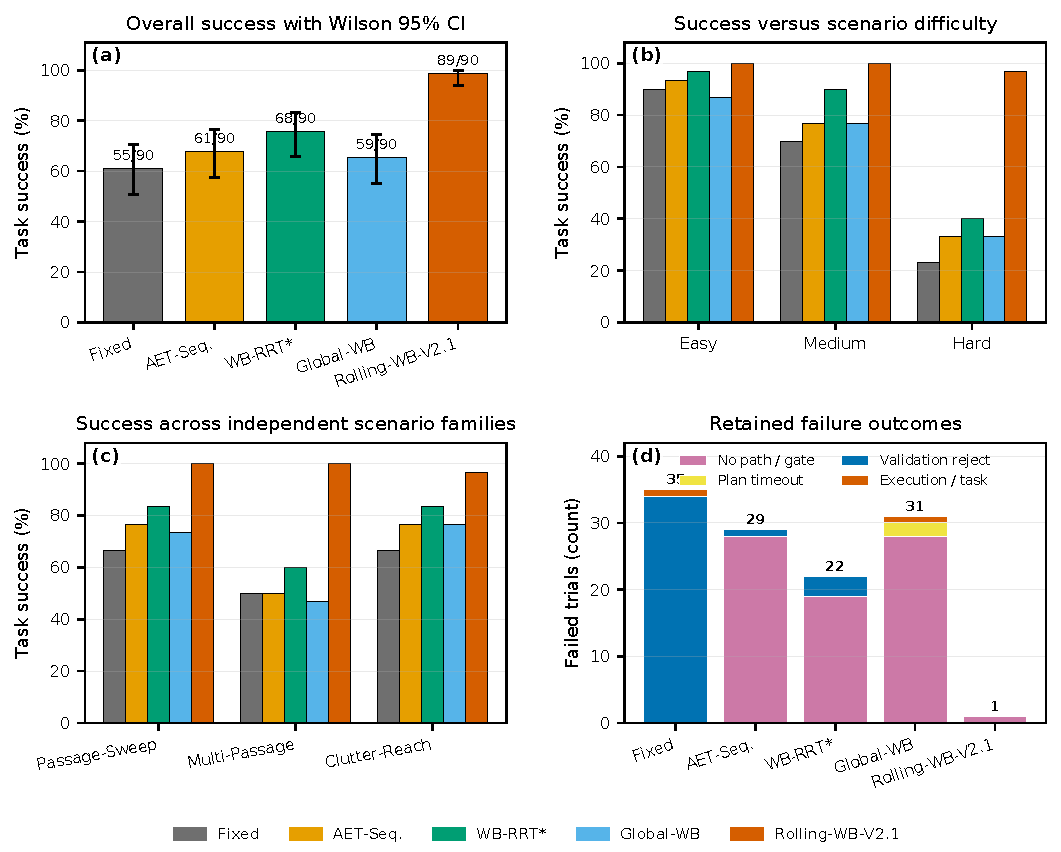
\includegraphics[width=0.88\textwidth]{outcomes_revised.pdf}
\caption{Task outcomes on the same 90 scenarios. (a) Overall success and Wilson 95\% intervals. (b) Success at each difficulty. (c) Success in each scenario family. (d) Retained failure categories. The single proposed-method failure arose from repeated candidate rejection beyond the registered threshold, not collision. Colors identify the same methods in all panels. The complete scenario-by-method outcome matrix is provided in Supplementary Fig.~S1.}
\label{fig:outcomes}
\end{figure*}

As shown in Table~\ref{tab:main} and Fig.~\ref{fig:outcomes}, \ours{} completed 89/90 tasks (98.9\%), compared with 68/90 (75.6\%) for WB-RRT*, an increase of 23.3 percentage points. On Hard tasks, success was 96.7\% versus 40.0\% for the strongest baseline. The proposed method completed every Passage-Sweep and Multi-Passage task and 29/30 Clutter-Reach tasks. Its only failure followed repeated gate rejection beyond the registered threshold; no collision was reported for that run.

\begin{table}[t]
\centering
\caption{Exact paired McNemar tests on the 90 tasks.}
\label{tab:mcnemar}
\small
\begin{tabular}{lrrc}
\toprule
Baseline & Ours only & Baseline only & Two-sided $p$\\\midrule
Fixed & 34 & 0 & $1.16\times10^{-10}$\\
AET-Seq. & 28 & 0 & $7.45\times10^{-9}$\\
WB-RRT* & 21 & 0 & $9.54\times10^{-7}$\\
Global-WB & 30 & 0 & $1.86\times10^{-9}$\\\bottomrule
\end{tabular}
\end{table}

% CN: 显著性限定为这组配对任务，不能替代更广泛环境泛化实验。
The discordant-pair counts in Table~\ref{tab:mcnemar} favored the proposed method on the matched task set, with no baseline-only successes. Planning latency had median 2.256~s and P95 3.697~s, and no attempt exceeded the 15-s deadline. Fixed was faster at P95, while the other planning baselines were slower. These measurements establish observed finite-budget computability on the tested platform, rather than a worst-case real-time guarantee.

\subsection{Execution Quality and Feasible-Space Use}
\begin{figure*}[!tb]
\centering
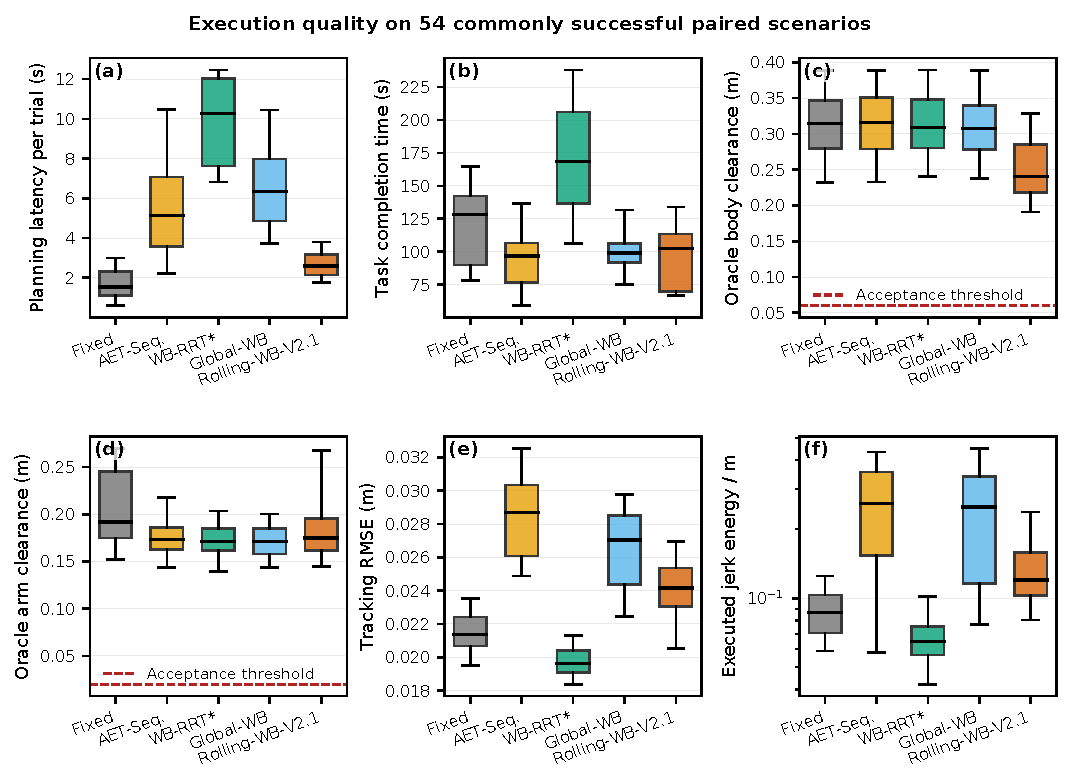
\includegraphics[width=0.94\textwidth]{quality_revised.pdf}
\caption{Continuous metrics on the 54 commonly successful tasks. (a) Planning latency, (b) task time, (c,d) audited body and arm clearance, (e) tracking RMSE, and (f) normalized jerk energy. Red dashed lines indicate post-hoc clearance thresholds; the logarithmic jerk scale is retained from the source. Pairing controls the evaluated task set but conditions the comparison on common success.}
\label{fig:quality}
\end{figure*}

% CN: 共同成功子集降低幸存者集合差异，但本身仍是条件分析，不能说完全消除选择偏差。
On the common-success subset (Fig.~\ref{fig:quality}), the proposed method's median planning latency was approximately 0.99~s above Fixed and 2.42, 6.49, and 3.64~s below AET-Seq., WB-RRT*, and Global-WB, respectively. The latter differences remained significant after Holm correction. This conditional comparison should be read alongside the all-task success results, because it excludes the harder tasks that some baselines failed.

Body-clearance paired median differences were approximately 5.4--6.2~cm below those of the baselines. The smaller separation indicates use of narrower feasible corridors while meeting the shared thresholds; it is not evidence of greater or lesser safety by itself. Arm-clearance differences were smaller and not consistently significant after correction. Tracking RMSE and normalized jerk were worse than Fixed and WB-RRT* but better than AET-Seq. and Global-WB. The observed advantage was primarily task feasibility under confined geometry, with a measurable computation and execution-quality tradeoff.

\subsection{Representative Passage and Rolling Updates}
\begin{figure*}[!tb]
\centering
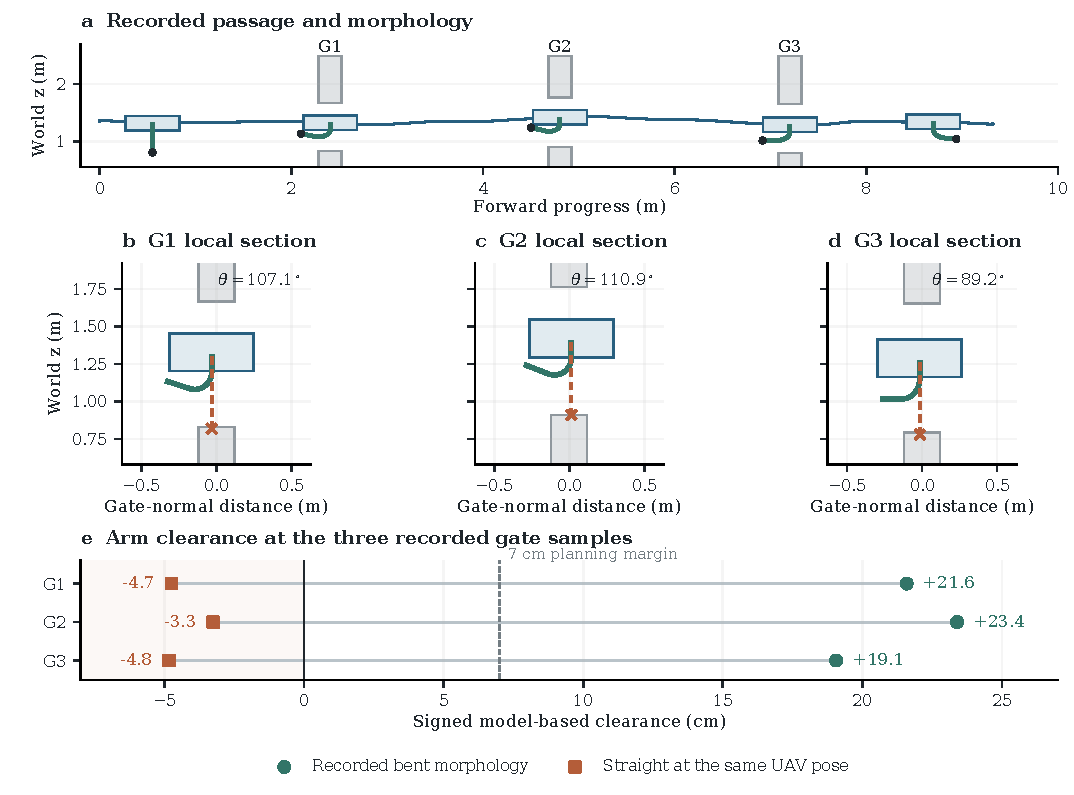
\includegraphics[width=\textwidth]{passage_mechanism_v2.pdf}
\caption{Morphology changes the geometric outcome in a recorded Multi-Passage task. (a) Side projection of the UAV path and five measured configurations; rectangles depict the body collision envelope. (b)--(d) Equal-scale gate-normal sections compare the recorded bent arm with a straight-arm counterfactual at the same UAV position and yaw. Crosses mark the counterfactual distal point. (e) Signed arm clearances at the three selected samples, computed with the frozen three-dimensional geometry; zero indicates contact and the dashed line marks the 7~cm planning margin. Samples are selected nearest each gate's world-$y$ center. Projections explain the mechanism; the audit uses the full three-dimensional boxes and sampled robot model.}
\label{fig:geometry}
\end{figure*}

Figure~\ref{fig:geometry} links the full passage to its local geometric constraints. The recorded bent configurations provide arm clearances of 21.6, 23.4, and 19.1~cm at G1--G3. Straightening the arm while retaining each measured UAV position and yaw changes these values to $-4.7$, $-3.3$, and $-4.8$~cm. Thus, the shape change alters the feasibility of the illustrated states, rather than merely changing the appearance of the path.

Increasing altitude alone also faces competing local constraints. With the original map inflation and planning margins, G1 requires a straight-arm UAV height of at least 1.465~m, whereas its upper-body constraint permits at most 1.422~m. The corresponding lower/upper height intervals are separated by 4.3, 2.3, and 2.0~cm at G1--G3. These are per-gate interval gaps for the specified local geometry, not collision depths or a restriction to constant altitude over the complete task. The counterfactual explains the demonstrated route; fixed-morphology planning with a newly optimized route is a separate comparison.

\begin{figure*}[!tb]
\centering
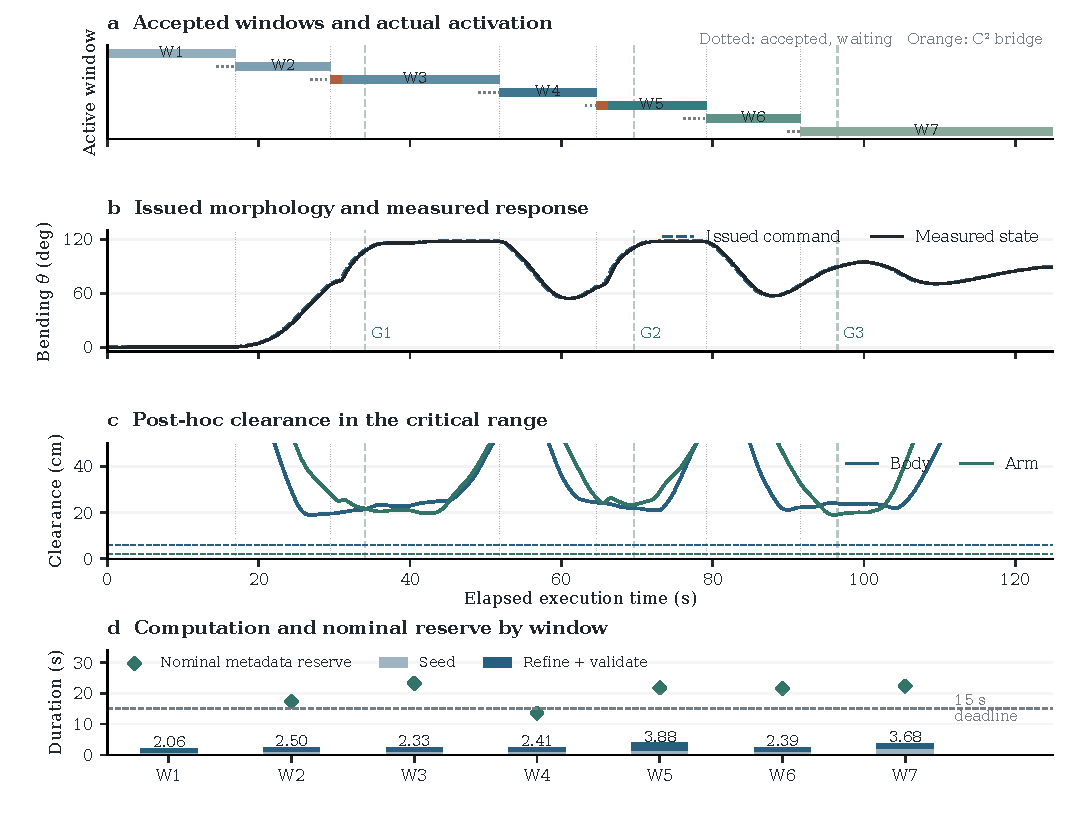
\includegraphics[width=\textwidth]{rolling_execution_v2.pdf}
\caption{Rolling execution reconstructed from the same recorded task. (a) Actual active-window intervals W1--W7; dotted segments indicate accepted successors awaiting activation, and orange segments denote the two 1.5~s validated C$^2$ bridges. (b) The actually issued bending command and measured bending response, rather than superseded candidate tails. (c) Post-hoc body and arm clearances, displayed over the critical 0--50~cm range; dashed horizontal lines are the original audit thresholds of 6 and 2~cm. Vertical dotted lines indicate activations; green dashed lines locate the samples used in Fig.~\ref{fig:geometry}. (d) Wall-clock computation durations and nominal reserve reconstructed from trajectory metadata, indexed by window. This reserve is not corrected for execution-phase modulation.}
\label{fig:rolling}
\end{figure*}

Figure~\ref{fig:rolling} separates planning, command issuance, and physical response. Seven accepted windows cover 124.96~s of task execution, with four direct successor handoffs and two revalidated C$^2$ bridges. The measured morphology follows the issued command while local candidates are replaced. Comparing execution with a superseded candidate tail would therefore not measure tracking error. The post-hoc sampled-model audit retains minimum body and arm clearances of 0.1889 and 0.1887~m over the recorded task.

Planning and validation require 2.06--3.88~s per window in this case, below the 15~s planning deadline. The nominal metadata reserves at successor acceptance are 13.5--23.3~s. Computation durations are plotted by window because solver wall time and execution timestamps have different time bases. Supplementary Fig.~S2 retains the additional position, bending-vector, and coupling histories, while Supplementary Fig.~S8 shows the full candidate plans, including portions superseded before execution.

\subsection{Handoff Continuity}


% CN: 候选缺口与相邻命令差不是同一物理统计量，不把二者直接相除当作因果改善率。
The benchmark recorded 391 handoffs: 339 passed the direct gate and 52 used a revalidated quintic bridge. Supplementary Fig.~S7 shows a representative transition, including the transient derivative peaks during bridging; it illustrates the issued commands rather than establishing a reduction in jerk by itself. Table~\ref{tab:handoff} separates the gap between candidate and active trajectories from the step between issued commands 50~ms apart. For example, bending-vector P95 was $22.7983^\circ$ for candidate gaps and $1.2358^\circ$ for issued steps. These are different diagnostic quantities; their comparison describes transition handling rather than a paired causal reduction ratio.

\begin{table}[t]
\centering
\caption{Transition diagnostics over 391 handoffs.}
\label{tab:handoff}
\footnotesize\setlength{\tabcolsep}{3pt}
\begin{tabular}{llrrrr}
\toprule
 & & \multicolumn{2}{c}{Candidate gap} & \multicolumn{2}{c}{50-ms issued step}\\
Metric & Unit & Median & P95 & Median & P95\\\midrule
Position & m & 0.0156 & 0.0549 & 0.0072 & 0.0306\\
Yaw & deg & 0.0039 & 0.0969 & 0.0014 & 0.0614\\
Bending vector & deg & 0.3243 & 22.7983 & 0.0423 & 1.2358\\
Linear velocity & m/s & 0.0077 & 0.0193 & 0.0039 & 0.0147\\
Linear acceleration & m/s$^2$ & 0.0195 & 0.0392 & 0.0064 & 0.0249\\\bottomrule
\end{tabular}
\end{table}

% CN: 72.8%按用户指定的配对统计结果保留，不用两个边际中位数反推此值。
A separate 15-scenario paired version comparison evaluated the earlier position-only switching implementation against the revised continuity-aware implementation. Both versions completed 15/15 tasks. The supplied paired analysis reported a 72.8\% median reduction in $E_{j/L}$, with improvement on all 15 tasks. This result characterizes the combined version change; an otherwise identical single-factor handoff ablation is needed to isolate the contribution of the gate and bridge.

\subsection{Morphology Feedback Under Visual Degradation}
% CN: 当前附件的图像明确写有指令推导/ORB拟合参考，故保留可核验的鲁棒性口径，不重命名为动捕真值。
Recorded-data stress tests evaluated whether fusion continued to track changing morphology as vision deteriorated. The supplied $\theta$ plot identifies a command-derived evaluation reference, while the $\phi$ plot identifies a normal-ORB-fitted reference. Figure~\ref{fig:sensing} retains their complete displayed angle trajectories. These references are distinct from the independent mocap labels used for strain calibration and do not establish absolute mocap-verified test accuracy.

\begin{figure*}[!tb]
\centering
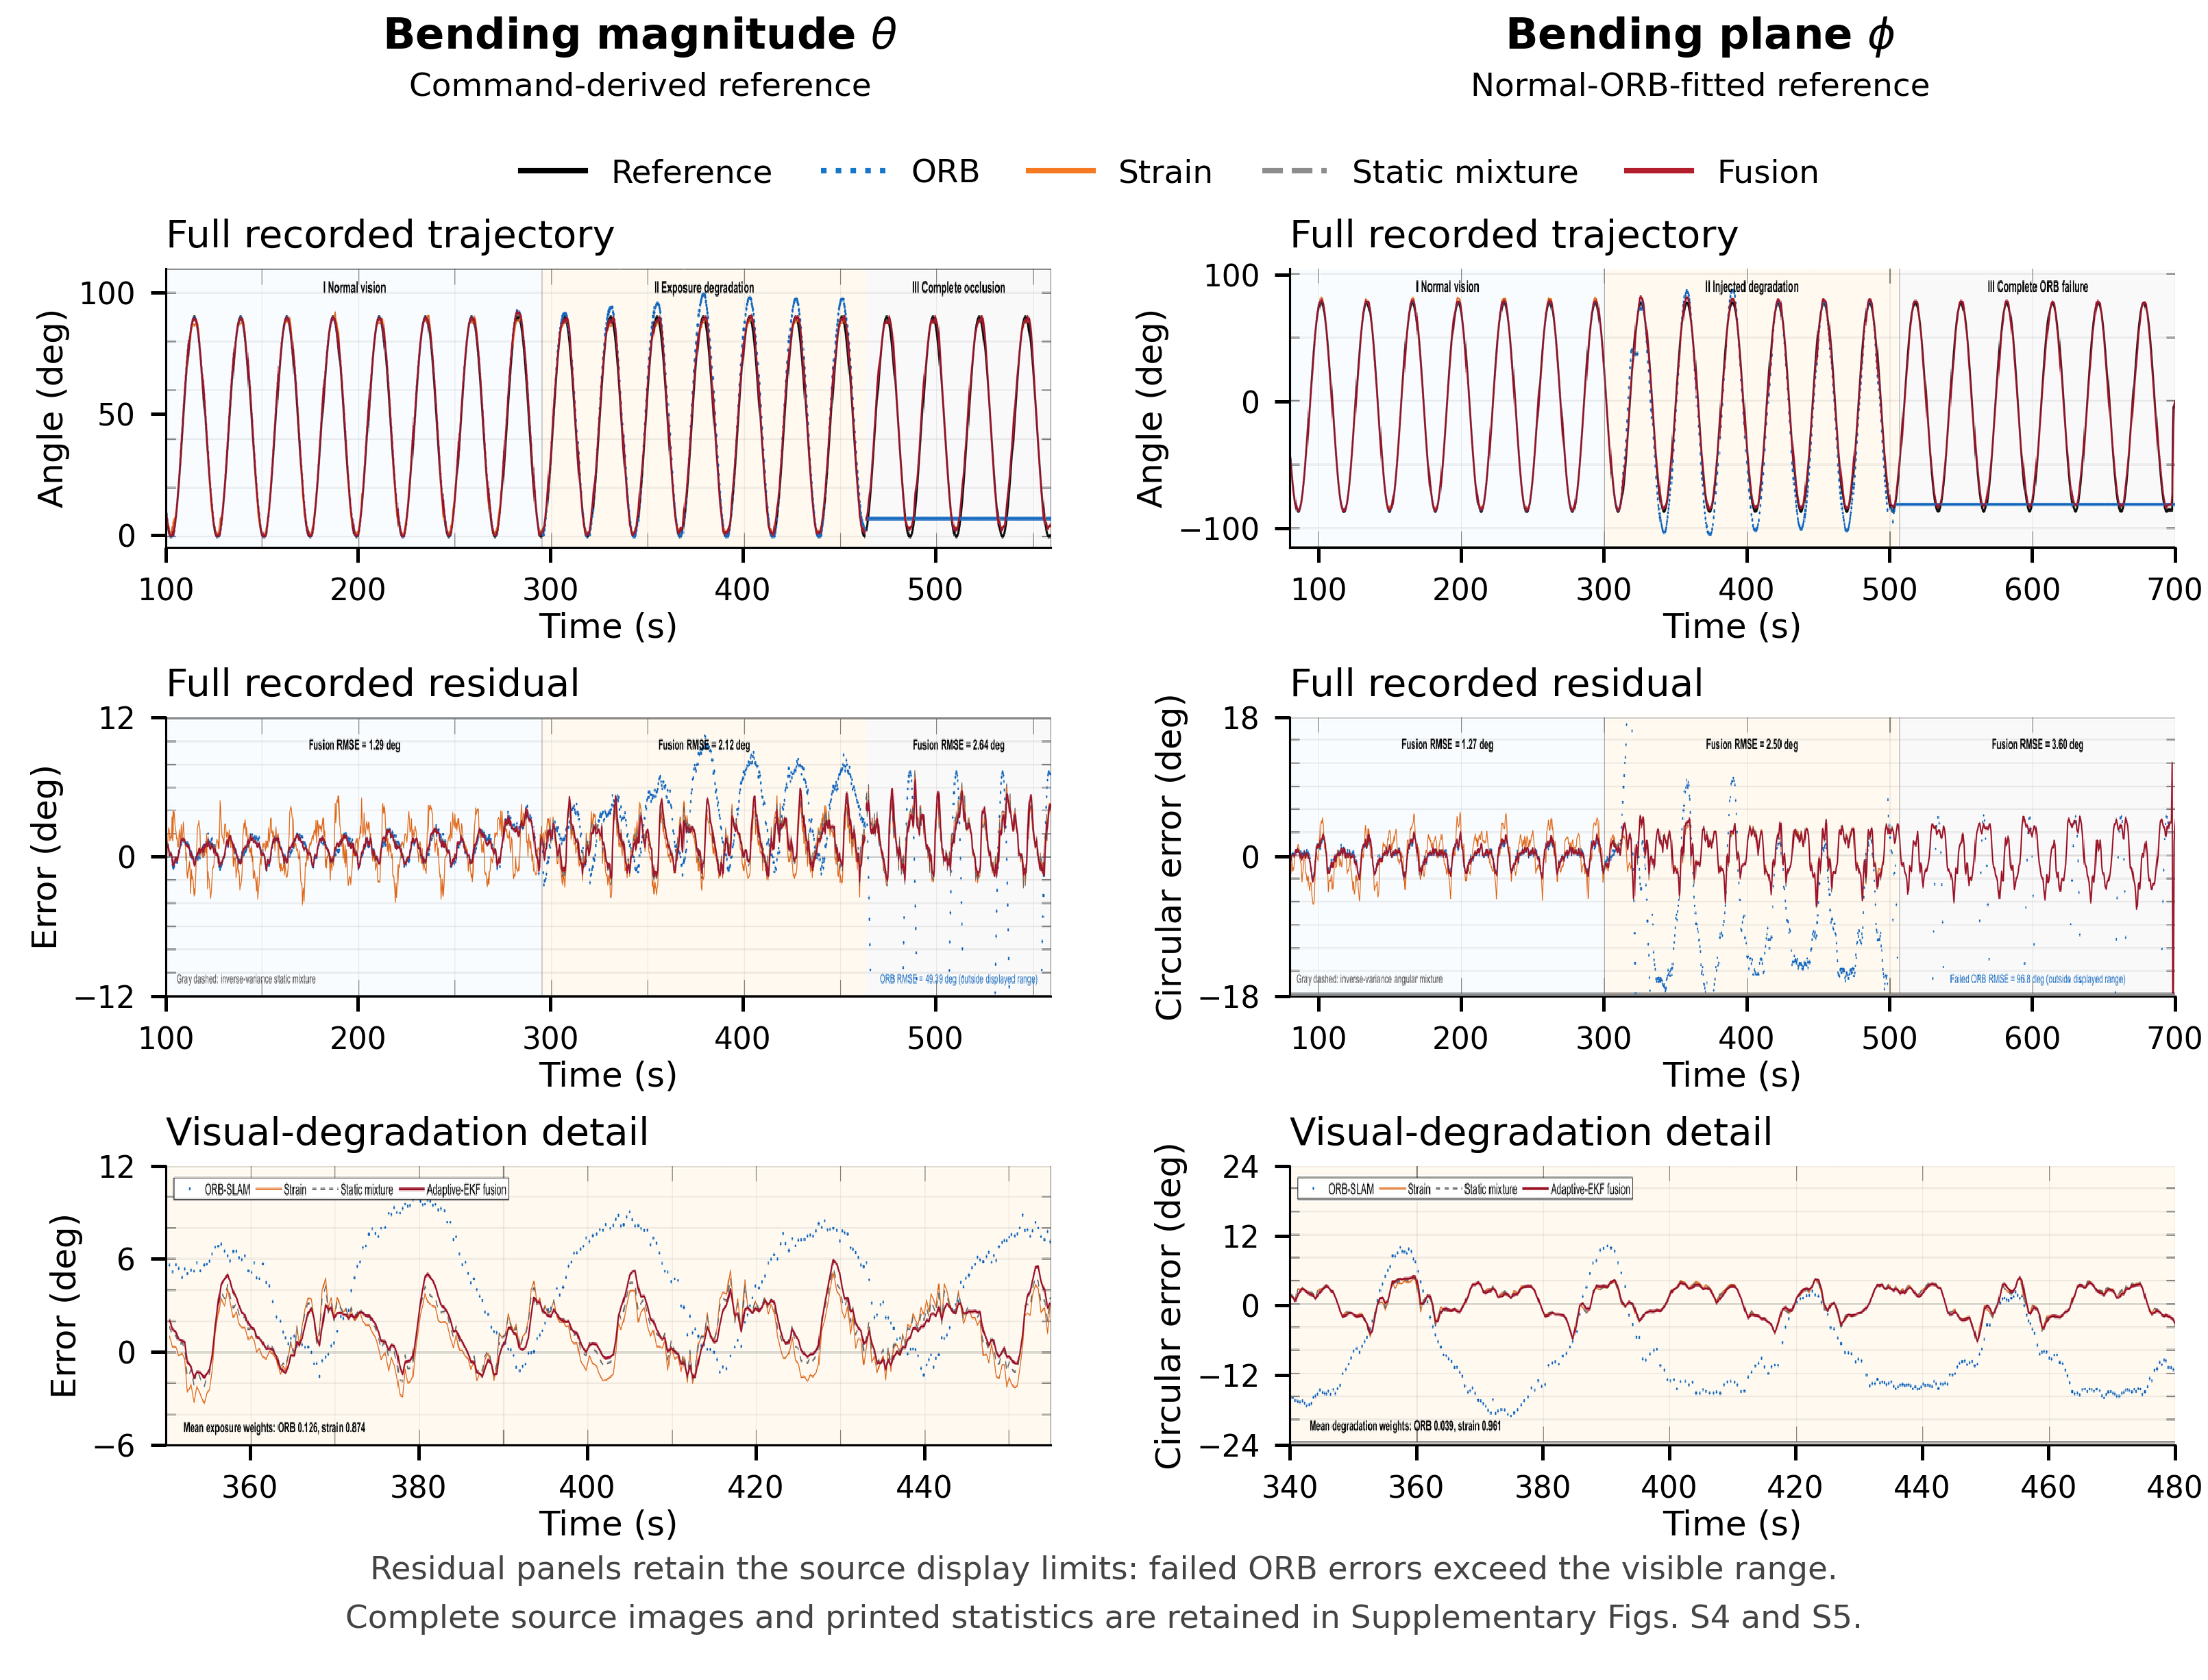
\includegraphics[width=\textwidth]{sensing_restored.png}
\caption{Recorded-data visual-degradation tests. Columns show bending magnitude and bending-plane angle; rows show full angle trajectories, full residual records, and enlarged degradation intervals. Black denotes the supplied reference, blue ORB, orange strain, gray static fusion, and red temporal fusion. The references are command-derived and normal-ORB-fitted, respectively. The source residual limits are retained: visual-loss errors extend beyond $\pm12^\circ$ for $\theta$ and $\pm18^\circ$ for $\phi$, so clipped visual residuals must not be interpreted as small errors. The source images and their printed statistics are preserved in Supplementary Figs.~S4 and S5.}
\label{fig:sensing}
\end{figure*}

\begin{table}[t]
\centering
\caption{Reported fusion errors relative to the supplied evaluation references (degrees).}
\label{tab:sensing}
\small
\begin{tabular}{lcc}
\toprule
Stage & $\theta$ RMSE & $\phi$ circular RMSE\\\midrule
Normal vision & 1.29 & 1.27\\
Degraded vision & 2.12 & 2.50\\
Complete visual loss & 2.64 & 3.60\\\bottomrule
\end{tabular}
\end{table}

Fusion errors increased gradually across the three stages (Table~\ref{tab:sensing}). Mean visual/strain weights in the highlighted degradation intervals were 0.126/0.874 for $\theta$ and 0.039/0.961 for $\phi$. Under complete loss, ORB-only errors reached approximately $49.4^\circ$ and $96.8^\circ$, whereas fusion remained at the strain-dominated error scale. The evidence supports modality reweighting and continued output during visual loss, without claiming that fusion outperforms every individual sensor in every condition.

\subsection{Flight-Load Proxies and Attribution}
% CN: PX4目标与实测姿态之间的统计不能直接当作规划倾角与实测之间的统计。
The supplied flight-response traces are provided in Supplementary Fig.~S3. Maximum realized tilt ranged from approximately $1.655^\circ$ to $2.345^\circ$, below the $15^\circ$ planning limit. Realized-versus-PX4-target tilt RMSE was $0.061^\circ$--$0.107^\circ$, with correlation 0.909--0.967. These statistics characterize attitude tracking; visual agreement with the planned tilt proxy is complementary evidence, not the same comparison.

The maximum thrust ratio was 1.0026--1.0058, consistent with near-hover motion. The proxy and low-pass IMU specific-force magnitude divided by $g$ differed by RMSE 0.0010--0.0011 but had weak temporal correlation ($-0.079$ to 0.167). IMU specific force is not a direct rotor-thrust measurement. The results therefore establish only low dynamic demand in the tested tasks, not accurate high-dynamic thrust prediction. The paired version comparison supports improved transition behavior without isolating each implementation change. The main success result belongs to the complete planning pipeline because separate seed and adaptive-plane ablations were not supplied.


\subsection{Hardware Demonstration of Morphology-Coordinated Execution}
\label{sec:hardware}
The simulation study examines the feasible-space benefit of joint morphology planning and the behavior of rolling trajectory transitions. We next demonstrate the corresponding morphology-coordination principle on the physical aerial continuum platform. The task connects passage traversal, target approach, object handling, and return flight in a shared scene, providing a physical counterpart to the confined-passage and terminal-reaching scenarios.

\begin{figure*}[!t]
\centering
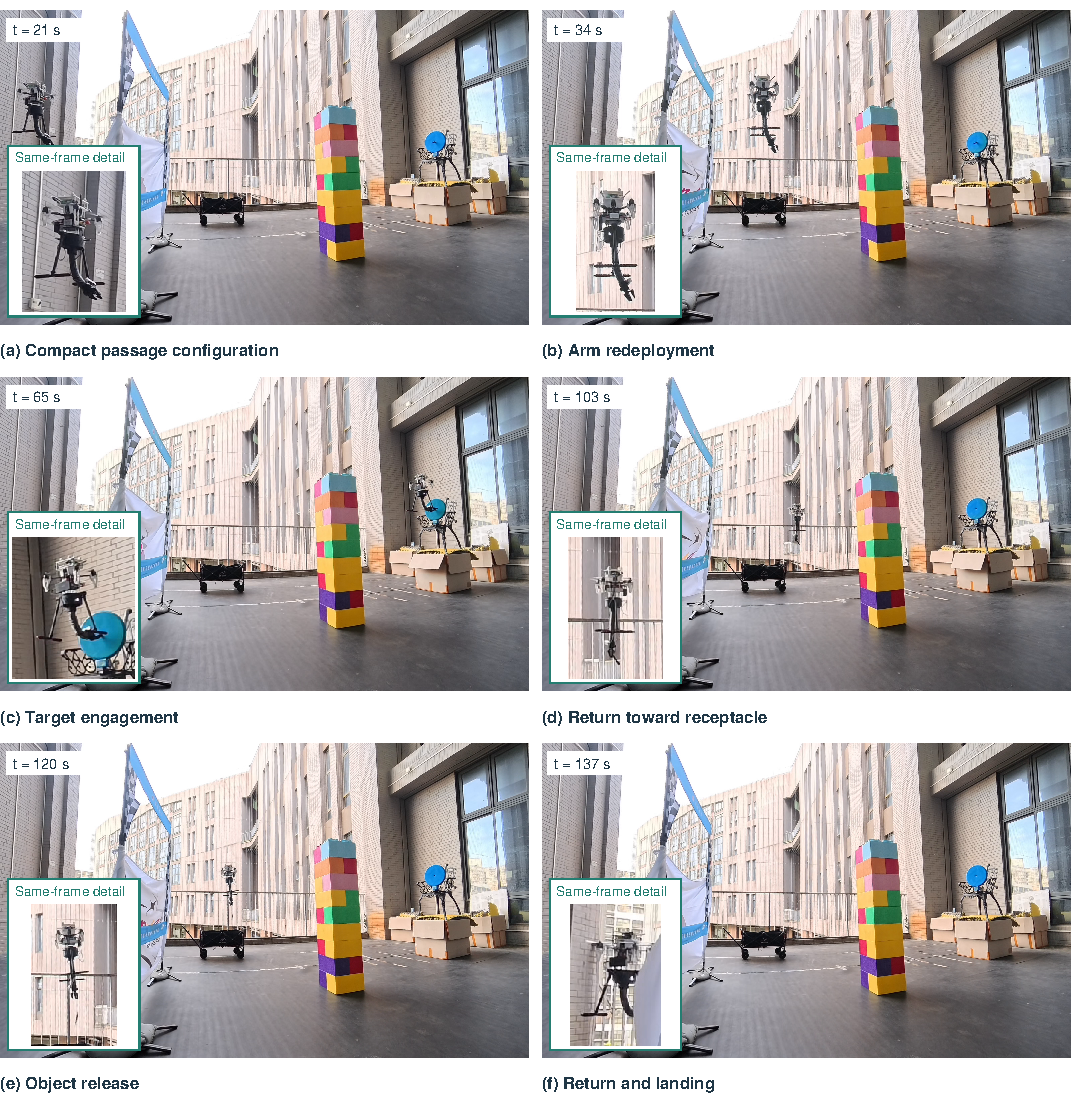
\includegraphics[width=\textwidth]{hardware_sequence_raw.pdf}
\caption{Physical demonstration of morphology-coordinated task execution. Frames sampled from one original video show (a) a compact configuration near the passage, (b) arm redeployment after passage, (c) target engagement, (d) return toward the receptacle, (e) object release, and (f) return and landing. Times refer to the source-video clock. All panels use the same scene crop; framed insets magnify the corresponding original frame. Robot and object shapes are preserved.}
\label{fig:hardware_sequence}
\end{figure*}

Figure~\ref{fig:hardware_sequence} presents the task sequence. The arm first adopts a compact configuration for passage and then redeploys to recover reach toward the target. Following target engagement, the vehicle returns toward the receptacle, releases the object, and returns to the landing area. The sequence illustrates the use of different continuum morphologies for transit and interaction within one task.

This physical sequence complements the simulation results at the level of task geometry: compact morphology accommodates the passage, whereas redeployment supports subsequent object interaction. The simulation comparisons quantify the planning mechanisms, and the hardware demonstration shows their physical task context.

% Draft-only reserved block. Populate it after the LiDAR-equipped re-flight.
\ifhardwareplaceholders
\begin{figure*}[!t]
\centering
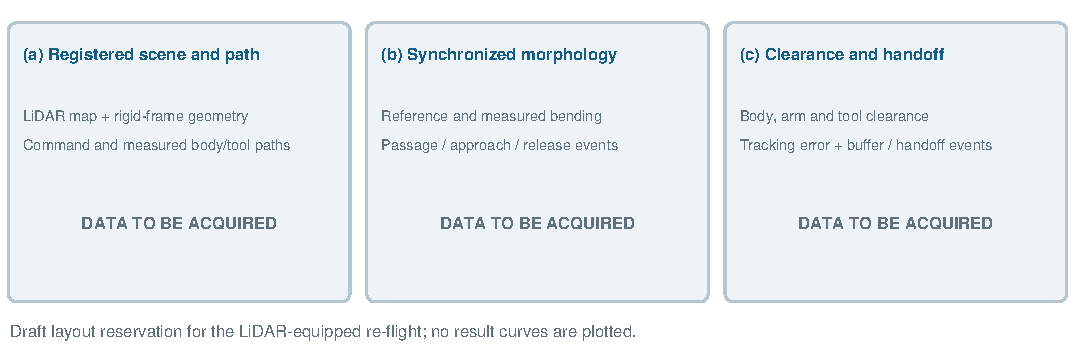
\includegraphics[width=\textwidth]{hardware_quantitative_slots.pdf}
\caption{Draft layout reserved for synchronized hardware evaluation: registered scene and trajectories, morphology tracking, and whole-body clearance with handoff events. Measurements will be inserted after the LiDAR-equipped re-flight.}
\label{fig:hardware_quantitative}
\end{figure*}
\begin{table}[t]
\centering
\caption{Draft hardware-evaluation fields for the planned re-flight.}
\label{tab:hardware_pending}
\small
\begin{tabular}{p{0.55\columnwidth}p{0.32\columnwidth}}
\toprule
Measure & Status\\\midrule
Attempts and completed tasks & To be acquired\\
Body / arm / tool minimum clearance & To be acquired\\
Position / bending tracking error & To be acquired\\
Planning latency and handoff events & To be acquired\\
Payload mass and release outcome & To be acquired\\\bottomrule
\end{tabular}
\end{table}
\fi


\section{Discussion}\label{sec:discussion}
% CN: 集中说明形态模型、采样几何及感知证据边界，避免在每段重复免责声明。
The useful operating regime is a single predominantly bending section in a static mapped environment under low-dynamic flight. Within this regime, morphology changes the usable corridor and must be planned jointly with vehicle motion. Nonuniform curvature, significant twist, rapid arm motion, and detailed camera/gripper housing geometry require richer modeling or a more conservative envelope. The yaw-only planning geometry and sampled distance checks limit the interpretation of acceptance; they do not provide a continuous-time or full-dynamics safety proof.

% CN: 贡献边界与实际验证相对应；给出缺口而不堆叠未来工作段落。
The experiments support different parts of the architecture at different levels. The planning benchmark demonstrates task feasibility and command-transition handling with a modeled morphology response. The recorded sensing study demonstrates graceful reweighting under visual degradation. The hardware demonstration illustrates the correspondence between compact passage morphology and redeployed interaction morphology in a physical task. A causal estimate of the benefit of visual--strain feedback to planning requires matched end-to-end trials. Independent mocap-referenced test traces are also needed to establish absolute sensing accuracy. These missing comparisons do not invalidate the observed planning results, but they delimit the claims that can be attributed to the complete architecture.

% CN: 计算预算、困难任务成功率与连续指标之间的取舍是讨论重点。
The planner trades extra computation and some execution smoothness against access to difficult corridors. It achieved higher success while Fixed and WB-RRT* retained better values on selected continuous metrics. Zero observed deadline misses does not imply a worst-case bound, and common-success analysis does not replace all-task evaluation. Likewise, finite-tolerance direct handoffs and derivative-matched command bridges should be judged by the disclosed command and task metrics rather than by unsupported physical continuity guarantees.

\section{Conclusion}\label{sec:conclusion}
% CN: 结论概括机制和证据，不重复完整摘要数据。
This work treats continuum morphology as a whole-body planning variable and separates local trajectory generation from execution authorization. Geometry-guided initialization and joint spline refinement address confined-space feasibility, while boundary inheritance and revalidated bridging manage the transitions created by rolling replanning. The paired benchmark showed that this combination improved difficult-task completion within the tested computation budget, and the paired version comparison showed improved transition behavior. A compatible visual--strain frontend maintained morphology output during visual loss in recorded-data tests. The hardware demonstration illustrates compact passage, arm redeployment, and subsequent object handling. Together, these results establish a modular basis for low-dynamic aerial continuum planning. Future work will quantify end-to-end hardware performance using synchronized onboard mapping, morphology, and trajectory records.

\appendices
\section{Development Checks for the New Simulation Backend}
The new backend is qualified separately from the historical benchmark. Its current eight-element, alternating-axis arm discretization was compared with the SDK-sized PCC reference at bending angles $0^\circ$, $30^\circ$, $60^\circ$, $90^\circ$, and $120^\circ$ in eight bending planes. The maximum endpoint and bending-vector errors were 2.136\,mm and $1.089^\circ$, respectively. These are numerical kinematic consistency checks, not errors measured on the physical robot.

Runtime commands and the new backend's planning model are limited to $118^\circ$, retaining a $2^\circ$ reserve below the $120^\circ$ evaluation bound. Four fixed-airframe actuator tests, each integrated for 14\,s in a different bending plane, produced a maximum total discrete curvature of $115.597^\circ$ with no evaluated step above $120^\circ$. Raw integrated states were retained without clipping. This test characterizes the current actuator model; stiffness, damping, friction, and mass properties still require physical identification before quantitative transfer claims.

The revised native CAD assembly is maintained as a distinct platform configuration. Its visual geometry, full rigid envelope including the landing gear, sensor extrinsics, and actuation model must be reconciled before it is used for closed-loop passage evaluation. Neither rendered CAD scenes nor these component checks are counted in the historical task-success statistics.

\balance
\bibliographystyle{IEEEtran}
\bibliography{references}
\end{document}
